\chapter{Paper 2: Null-sampling for Interpretable and Fair Representations}\label{ch:paper2}
% \documentclass[runningheads]{llncs}
% \pdfoutput=1
% \usepackage[utf8]{inputenc}
% \usepackage{graphicx}
% \usepackage{comment}
% \usepackage{biblatex}
% \usepackage{placeins}
% \usepackage{amsmath,amssymb,amsfonts,bm} % define this before the line numbering.
% \usepackage{color}
% \usepackage{booktabs}

% \usepackage{import}
% \usepackage{appendix}
% \usepackage[caption=false]{subfig}
% \usepackage{mathtools}
% \usepackage{wrapfig}
% \usepackage{hyperref}

% \def\ci{\perp\!\!\!\perp}
% \newcommand*\diff{\mathop{}\!\mathrm{d}}
% \def\httilde{\mbox{\tt\raisebox{-.5ex}{\symbol{126}}}}

% \addbibresource{references.bib}

% \begin{document}

% \pagestyle{headings}
% \mainmatter
% \def\ECCVSubNumber{5488}  % Insert your submission number here

% \title{Null-sampling for Interpretable \\and Fair Representations} % Replace with your title

% \titlerunning{Null-sampling for Interpretable and Fair Representations}
% \author{Thomas Kehrenberg \and
% Myles Bartlett \and
% Oliver Thomas \and \\
% Novi Quadrianto}
% \authorrunning{T. Kehrenberg et al.}
% \institute{Predictive Analytics Lab (PAL), University of Sussex, Brighton, UK
% \email{\{t.kehrenberg,m.bartlett,ot44,n.quadrianto\}@sussex.ac.uk}}
% \maketitle

\textsc{Authors}:\\
Thomas Kehrenberg$^1$, Myles Bartlett$^1$, Oliver Thomas$^1$, and Novi Quadrianto$^1$ \\
\textsc{Affiliations}:\\
$^1$ Predictive Analytics Lab (PAL), University of Sussex, Brighton, UK\\
\textsc{Conference}:\;\;\textit{European Conference on Computer Vision} (ECCV), 2020 \\
\textsc{DOI}:\;\;\texttt{10.1007/978-3-030-58574-7\_34} \\
\textsc{Note}:\;\;The appendix has been included as section~\ref{sec:nifr-appendix}.

% 70-150 words
\section{Abstract}
\noindent
% Training data often contains spurious correlations not reflected in the real world where a trained model will be deployed.
% Consequently, computer vision and machine learning systems can become over-reliant on these correlations for classifications.
% Instead of basing their output on those features which are semantically meaningful, the output can be based on these unintended relationships.
% This is undesirable for many reasons, among them limited generalisation and uncontrolled bias.
We propose to learn invariant representations, in the data domain, to achieve interpretability in algorithmic fairness. 
Invariance implies a selectivity for high level, relevant correlations w.r.t.\ class label annotations, and a robustness to irrelevant correlations with protected characteristics such as race or gender. 
We introduce a non-trivial setup in which the training set exhibits a strong bias such that class label annotations are irrelevant and spurious correlations cannot be distinguished.
To address this problem, we introduce an adversarially trained model with a \emph{null-sampling} procedure to produce invariant representations in the data domain.
To enable disentanglement, a partially-labelled \emph{representative} set is used.
By placing the representations into the data domain, the changes made by the model are easily examinable by human auditors.
We show the effectiveness of our method on both image and tabular datasets: Coloured MNIST, the CelebA and the Adult dataset.%
% At the same time, it is important the people be able to trust the outputs of machine learning systems 
% To address this problem, we propose dividing training into a straightforward and general two-step procedure.
% In this framework, the model is first trained to produce invariant representations from an unlabelled pre-training set, in which there exists minimal spurious correlations.
% In the second step a classifier is trained on the encoding generated for the biased training set.
% We first demonstrate the viability of our  No Shortcuts in Neural Network (NoSiNN) framework with a AutoEncoder model before showing how its drawbacks can be ameliorated through the use of an Invertible architecture.
% Experiments with face images, coloured digits, and census data show promising results in decorrelating the spurious and non-spurious semantic features.

\section{Introduction}
% We need to stare start with something with more punch
%r rather than just a f matter-of-fact statement
%Fair representations are a means of removing potentially sensitive information from training data
%in order to avoid wrongly relying on the sensitive information for classification.

Without due consideration for the data collection process, machine learning algorithms can exacerbate biases, or even introduce new ones if proper control is not exerted over their learning \cite{holstein2019improving}. 
While most of these issues can be solved by
% While efforts should be made to
controlling and curating data collection in a fairness-conscious fashion, 
% aiming to eliminate algorithmic bias during the early stages of the pipeline, 
doing so is not always an option, such as when working with historical data.
Efforts to address this problem algorithmically have been centred on developing statistical definitions of fairness and learning models that satisfy these definitions.
One popular definition of fairness used to guide the training of fair classifiers, for example, is \emph{demographic parity}, stating that positive outcome rates should be equalised (or \emph{invariant}) across protected groups.

In the typical setup, we have an input $\bm{x}$, a sensitive attribute $s$ that represents some non-admissible information like gender
and a class label $y$ which is the prediction target.
The idea of fair \emph{representation} learning \cite{ZemWuSwePitetal13}\cite{edwardsstorkey}\cite{madras2018learning}
is then to transform the input $\bm{x}$ to a representation $\bm{z}$ which is invariant to $s$.
Thus, learning from $\bm{z}$ will not introduce a forbidden dependence on $s$.
% $\bm{z}$ can then be used to learn a predictor
% In fair representation learning \cite{ZemWuSwePitetal13}\cite{edwardsstorkey}\cite{madras2018learning}, the goal is then to find a representation $\bm{z}$ that is invariant to $s$.
A good fair representation is one that preserves most of the information from $\bm{x}$ while satisfying the aforementioned constraints.
% While fair \emph{representations} are by no means the only method of achieving this goal, approaches that explicitly depend on the target label \cite{kamiran2012data} are restrictive in that they do not readily admit transfer to unseen tasks, and are bound by the requirement of having $s$ and $y$ labels be present together.

As unlabelled data is much more freely available than labelled data, it is of interest to learn the representation in an unsupervised manner.
This will allow us to draw on a much more diverse pool of data to learn from.
% ; this is particularly pertinent for fair representation learning as unlabelled data affords us a much more diverse pool of data to learn from.
%To this end, \cite{locatello2019fairness} recently made the connection from disentangled representations to fair representations:
%a model for disentanglement trained without knowledge of the sensitive attribute $s$
%nevertheless appears to improve fairness measures with respect to $s$.
%However, as pointed out by \cite{locatello2019challenging},
%some supervision or inductive bias is needed in order to recognise a well-disentangled representation.
While annotations for $y$ are often hard to come by (and often noisy \cite{KehCheQua18}),
annotations for the sensitive attribute $s$ are usually less so, as $s$ can often be obtained from demographic information provided by census data.
We thus consider the setting where the representation is learned from data
that is only labelled with $s$ and not $y$.
This is in contrast to most other representation learning methods.
% We thus consider the setting where data labelled with $s$ (partially labelled data) is available for learning the fair representation.
% Furthermore, we assume the existence of a set with $s$ labels
% whose distribution matches the deployment setting
We call the set used to learn the representation the \emph{representative} set,
because its distribution is meant to match the distribution of the deployment setting
(and is thus representative).
% We call this set the \emph{representative} set and its distribution is meant to match the distribution of the deployment setting.

Once we have learnt the mapping from $\bm{x}$ to $\bm{z}$,
we can transform the \emph{training} set which, in contrast to the representative set, has the $y$ labels (and $s$ labels).
In order to make our method more widely applicable,
we consider an \emph{aggravated fairness problem}
% we allow the case
in which the training set contains a strong spurious correlation between $s$ and $y$,
which makes it impossible to learn from it a representation which is invariant to $s$ but not invariant to $y$.
Non-invariance to $y$ is important in order to be able to predict $y$.
The training set thus does \emph{not} match the deployment setting,
thereby rendering the representative set essential for learning the right invariance.
% We also tackle the related problem of learning from biased data, specifically cases in which the training set (with $y$ labels) contains a strong spurious correlation between $s$ and $y$, and thus does not match the deployment setting.
From hereon, we will use the terms \emph{spurious} and \emph{sensitive} interchangeably, depending on the context, to refer to an attribute of the data we seek invariance to.
% This is essentially a form of strong sampling bias and is not an unrealistic complication, having been shown to plague real-world datasets \cite{kallus2018residual}.
%Classifiers trained on ImageNet for example, have been shown to be biased towards texture \cite{Geir18}. \cite{zhang2018visual} similarly examine the problem of learning from biased data, showing that pre-trained models can exploit biases in the data by learning patterns semantically unrelated to the target, an issue that can be difficult to identify when the bias pervades both the training and test sets.
We can draw a connection between learning in the presence of spurious correlations and what \cite{kallus2018residual} call \emph{residual unfairness}.
Consider the Stop, Question and Frisk (SQF) dataset for example:
the data was collected in New York City, but the demographics of the recorded cases do not represent the true demographics of NYC well.
The demographic attributes of the recorded individuals might correlate so strongly with the prediction target that the two are nearly indistinguishable.
This is the scenario that we are investigating: $s$ and $y$ are so closely correlated in the labelled dataset that they cannot be distinguished, but the learning of $s$ is favoured due to being the ``path of least resistance''.
The deployment setting (i.e.\ the test set) does not possess this strong correlation and thus a na\"ive approach will lead to very unfair predictions.
In this case, a disentangled representation is insufficient;
the representation needs to be explicitly invariant solely with respect to $s$.
In our approach, we make use of the (partially labelled) representative set to learn this invariant representation.

While there is a substantial body of literature devoted to the problems of fair representation-learning, exactly how the invariance in question is achieved is often overlooked. 
When critical decisions, such as who should receive bail or be released from jail, are being deferred to an automated decision making system, it is critical that people be able to trust the logic of the model underlying it, whether it be via semantic or visual explanations. 
We build on the work of \cite{QuaShaTho19} and learn a decomposition ($f^{-1}: Z_s \times Z_{\neg s} \rightarrow X$) of the \emph{data domain} ($X$) into independent subspaces \emph{invariant} to  $s$ ($Z_{\neg s}$) and \emph{indicative} of $s$ ($Z_{s}$), which lends an interpretability that is absent from most representation-learning methods.
While model interpretability has no strict definition \cite{zhang2018visual}, we follow the intuition of \cite{adel2018discovering} -- \emph{a simple relationship to something we can understand}, a definition which representations in the data domain naturally fulfil.

Whether as a result of the aforementioned sampling bias or simply because the features necessarily co-occur, it is not rare for features to correlate with one another in real-world datasets.
Lipstick and gender for example, are two attributes that we expect to be highly correlated and to enforce invariance to gender can implicitly enforce invariance to makeup.
This is arguably the desired behaviour.
However, unforeseen biases in the data may engender cases which are less justifiable.
By baking interpretability into our model (by having representations in the data domain), though we still have no better control over what is learned, we can at least diagnose such pathologies.

To render our representations interpretable, we rely on a simple transformation we call \emph{null-sampling} to map invariant representations in the data domain.
Previous approaches to fair representation learning \cite{beutel,edwardsstorkey,madras2018learning,LouSweLi15} predominantly rely upon autoencoder models to jointly minimise reconstruction loss and invariance.
We discuss first how this can be done with such a model that we refer to as cVAE (conditional VAE),
before arguing that the bijectivity of invertible neural networks (INNs)~\cite{Dinh2014} makes them better suited to this task. 
We refer to the variant of our method based on these as cFlow (conditional Flow).
INNs have several properties that make them appealing for unsupervised representation learning. 
The focus of our approach is on creating invariant representations that preserve the non-sensitive information maximally, with only knowledge of $s$ and not of the target $y$, while at the same time having the ability to easily probe what has been learnt.

% The problem of fair representations can also be viewed through a similar lens.
% A good toy model for this setup is the Coloured MNIST (cMNIST) dataset.
% In this example, the colour is a spurious variable which is very closely correlated with the prediction target in the training set but not in the deployment setting.
% An interpretable invariant representation in this case is the images uniform in colour. More details regarding the setup and synthesis of the dataset can be found in Section~\ref{ssec:cmnist}.

% As a more real-world dataset, we consider the CelebA dataset.
% We treat the CelebA dataset as it is, as the deployment setting
% and construct deliberately biased subsets of CelebA to serve as the training set.
% In our experiments we use gender as the sensitive attribute.
% Sample images can be seen in \thomas{Fig.??}.
% Attributes that are correlated with gender in the \emph{deployment setting} (like the use of lipstick) will also be removed by our method.
% We do not consider this a defect of our method and instead argue that this is the correct behaviour:
% As long as the deployment setting is sufficiently diverse, the model may make use of correlations found in there.
%wearing lipstick is a valid indicator of gender.
%\thomas{maybe don't include the previous sentence}

Our contribution is thus two-fold:
1) We propose a simple approach to generating representations 
% through use of an INN, 
that are invariant to a feature $s$, while having the benefit of interpretability that comes with being in the data domain.
We call our model \emph{NIFR} (\textbf{N}ull-sampling for \textbf{I}nterpretable and \textbf{F}air \textbf{R}epresentations).
2) We explore a setting where the labelled training set suffers from varying levels of sampling bias,
% which we expect to be common not only in fairness problems but machine learning problems more broadly,
demonstrating an approach based on transferring information from a more diverse representative set,
with guarantees of the non-spurious information being preserved.

\begin{figure*}[tb]
  \centering
  \subfloat[Original images.]{%
      \scalebox{0.3}{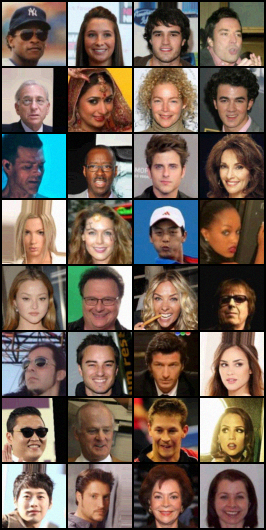
\includegraphics[width=\textwidth]{./Images/celeba/train_original_x_2.png}}%
      \label{fig:cflow_celeba_original_x}
  }
  \hfill
  \subfloat[$\bm{x}_u$ null-samples from the cFlow model.]{%
      \scalebox{0.3}{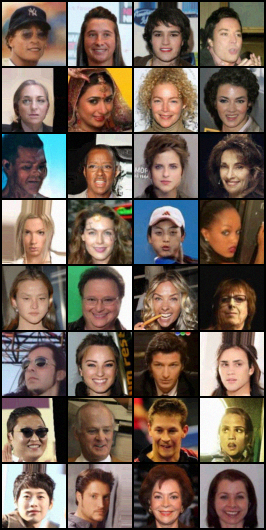
\includegraphics[width=\textwidth]{./Images/celeba/train_reconstruction_y_2.png}}%
      \label{fig:cflow_celeba_recon_y}
  }
  \hfill
  \subfloat[$\bm{x}_b$ null-samples from the cFlow model.]{%
      \scalebox{0.3}{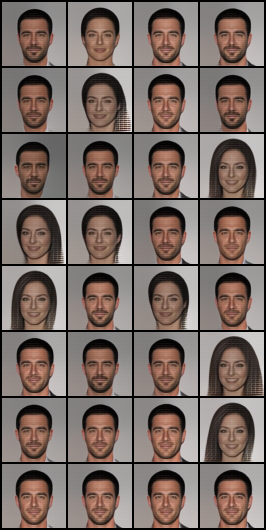
\includegraphics[width=\textwidth]{./Images/celeba/train_reconstruction_s_2.png}}%
      \label{fig:cflow_celeba_recon_s}
  }
  \caption{
    CelebA null-samples learned by our cFlow model, with gender as the sensitive attribute.
    (a) The original, untransformed samples from the CelebA dataset
    (b) Reconstructions using only information unrelated to $s$.
    (c) Reconstruction using only information related to $\neg s$.
    The model learns to disentangle gender from the non-gender related information.
    % Attributes such as \emph{makeup} and \emph{hair length} are also often modified in the process due to inherent correlations between them and the sensitive attribute, which the intepretability of our representations allows us to easily identify.
    Note that some attributes like skin tone seem to change along with gender due to the correlation between the attributes.
    This is especially visible in images (1,1) and (3,2). Only because our representations are produced in the data-domain can we easily spot such instances of entanglement.
  }%
  \label{fig:celeba_cflow}
\end{figure*}

\begin{figure*}[!htb]
    \centering
    \subfloat[Samples from the cMNIST training set, $\sigma=0$.]{%
        \scalebox{0.3}{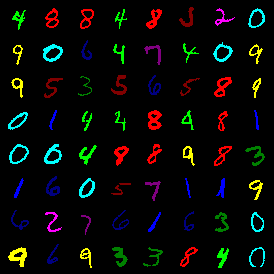
\includegraphics[width=\textwidth]{paper2/Images/cmnist/cflow_original_task_x_scale_0.png}}%
        \label{fig:cflow_cmnist_task_train}
    }
    % \hfill
    % \subfloat[Samples from the cMNIST test set with $\sigma=0.02$.]{%
    %     \scalebox{0.225}{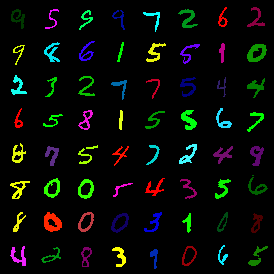
\includegraphics[width=\textwidth]{./Images/cmnist/cflow_pretrain_x.png}}%
    %     \label{fig:cflow_cmnist_pretrain}
    % }
    \hfill
    \subfloat[$x_u$ null-samples from the cFlow model.]{%
        \scalebox{0.3}{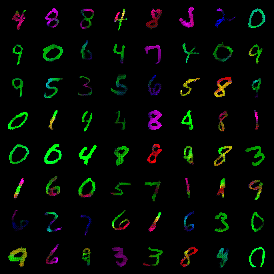
\includegraphics[width=\textwidth]{paper2/Images/cmnist/cflow_task_xy_scale_0.png}}%
        \label{fig:cflow_cmnist_y}
    }
    \hfill
    \subfloat[$x_b$ null-samples from the cFlow model.]{%
        \scalebox{0.3}{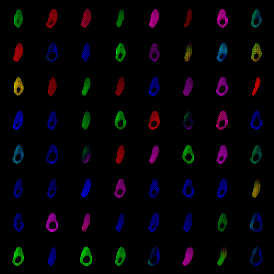
\includegraphics[width=\textwidth]{paper2/Images/cmnist/cflow_task_xs_scale_0.png}}%
        \label{fig:cflow_cmnist_s}
    }
    \caption{
        Sample images from the coloured MNIST dataset problem with $10$ predefined mean colours.
        (a): Images from the spuriously correlated subpopulation where colour is a reliable signal of the digit class-label.
        (b-c): Results of running our approach realised with cFlow on the cMNIST dataset.
        The model learns to retain the shape of the digit shape while removing the relationship with colour.
        A downstream classifier is now less prone to exploiting correlations between colour and the digit label class.
    }\label{fig:cmnist}
\end{figure*}


\section{Background}\label{sec:background}
% \noindent We frame our approach in the context of relevant literature on the interrelated problems of fair representation learning and learning representations free of spurious correlations.
% The background is far too long - we also need to touch on the interpretability literature

\subsection{Learning fair representations.}
%As we have alluded to, the goal of producing invariant representations is similar to that of producing \emph{fair} representations.
% In fairness problems, there is usually a \emph{sensitive attribute}, $s$ (for example, gender or race),
% that should not be used to make decisions.
Given a sensitive attribute $s$ (for example, gender or race) and inputs $\bm{x}$,
a fair representation $\bm{z}$ of $\bm{x}$ is then one for which $\bm{z} \perp s$ holds,
while ideally also being predictive of the class label $y$.
\citet{zemel2013learning} was the first to propose the learning of fair representations which allow for transfer to new classification tasks.
More recent methods are often based on \acfp{VAE}~\citep{kingma2013auto,louizos2016variational,edwards2016censoring,beutel2017data}.
The achieved fairness of the representation can be measured with various fairness metrics.
These measure, however, usually how fair the predictions of a classifier are
and not how fair a representation is.
% defined with respect to predictions and not representations.

% There is not one metric universally best-suited to measuring the invariance (or fairness) of representations.
The appropriate measure of fairness for a given task is domain-specific \citep{liu2018delayed}
and there is often not a universally accepted measure.
However, \emph{Demographic Parity} is the most widely used~\citep{louizos2016variational,edwards2016censoring,beutel2017data}.
Demographic Parity demands $\hat{y} \perp s$ where $\hat{y}$ refers to the predictions of the classifier.
In the context of fair representations, we measure the Demographic Parity of a downstream classifier, $f(\cdot )$, which is trained on the representation $z$, i.e.\  $f: Z \to \hat{Y}$.

A core principle of all fairness methods is the \emph{accuracy-fairness trade-off}.
As previously stated, the fair representation should be invariant to $s$ ($\to$ fairness) but still be predictive of $y$ ($\to$ accuracy).
These desiderata cannot, in general, be simultaneously satisfied if $s$ and $y$ are correlated.
% We explore this trade-off with our method as well. % DO WE?!?!?!?!?


The majority of existing methods for fair representations also make use of $y$ labels during training,
in order to ensure that $\bm{z}$ remains predictive of $y$.
This aspect can, in theory, be removed from the methods,
but then there is no guarantee that information about $y$ is preserved \citep{louizos2016variational}. 
% Existing methods designed to create fair representations can, in theory, be extended to the regime in which only the $s$, and not the $y$, labels are available. 
% However, it is not without its drawbacks as, in removing $s$, there is no guarantee that information about $y$ is preserved \cite{louizos2016variational}. 
% For this reason, $y$ is typically supplied during training and the representation encouraged to be predictive of it.

\subsection{Learning fair, transferrable representations}
% Outside of computer vision, \cite{madras2018learning} have also worked on removing a problematic spurious correlation.
In addition to producing fair representations, \citet{madras2018learning} want to ensure the representations are transferrable.
Here, an adversary is used to remove sensitive information from a representation $z$.
Auxiliary prediction and reconstruction networks, to predict class label $y$
% to ensure it remains predictive of $y$
and reconstruct the input $x$ respectively,
are trained on top of $z$, with $s$ being ancillary input to the reconstruction.
% alongside a reconstruction loss computed with respect to the output of a decoder that takes $z$ and the sensitive label $s$ as input is added. 
% This is so that $x$ can still be reconstructed from $z$, despite the removal of $s$.
%The decoder is utilised only for the purpose of maximum likelihood learning of the data distribution.
% By conditioning the decoder on the sensitive attribute, information about it can be ``off-loaded'' from the encoder such that information about $s$ need not be contained in the fair representation while still permitting the use of a reconstruction loss needed to capture non-sensitive information.
% The decoder plays a role only in the loss function.
% In contrast, we make explicit use of the decoder not only for characterising the behaviour of the model and also for evaluation.

Also related is \citet{creager2019flexibly} who employ a FactorVAE \citep{kim2018disentangling} regularised for fairness.
The idea is to learn a representation that is both disentangled and invariant to multiple sensitive attributes.
This factorisation makes the latent space easily manipulable such that the different subspaces can be freely removed and composed at test time.
Zeroing out the dimensions or replacing them with independent noise imparts invariance to the corresponding sensitive attribute.
This method closely resembles ours when we use an invertible encoder.
However, the emphasis of our approach is on interpretability, information-preservation, and coping with sampling bias - especially extreme cases where $|\, \textrm{supp}(S_{tr} \times Y_{tr}) | < |\, \textrm{supp}(S_{te} \times Y_{te}) |$.
% Namely, the invertibility of the network means we can optimise for invariance singularly without the burden of a reconstruction loss.
% While we do not explicitly consider the case of multi-attribute fairness, our method can be easily adapted for this use-case.

Attempts were made by~\citet{QuaShaTho19} prior to this work to learn fair representations in the data domain in order to make it interpretable and transferable.
In their work, the input is assumed to be additively decomposable in the feature space into a \emph{fair} and \emph{unfair} component, which together can be used by the decoder to recover the original input.
This allows us to examine representations in a human-interpretable space and confirm that the model is not learning a relationship reliant on a sensitive attribute.
Though a first step in this direction, we believe such a linear decomposition is not sufficiently expressive to fully capture the relationship between the sensitive and non-sensitive attributes.
Our approach allows for the modelling of more complex relationships.

\subsection{Learning in the presence of spurious correlations}
% As  previously  discussed,  the  goal  of  producing  fair representations is similar to the goal of producing representations invariant to spurious correlations found in the training data.
Strong spurious correlations make the task of learning a robust classifier challenging: the classifier may learn to exploit correlations unrelated to the true causal relationship between the features and label, and thereby fail to generalise to novel settings.
This problem was recently tackled by \citet{kim2019learning} who apply a penalty based on the mutual information between the feature embedding and the spurious variable. 
While the method is effective under mild biasing, we show experimentally that it is not robust to the range of settings we consider.

\citet{JacBehZemBet19} explore the vulnerability of traditional neural networks to spurious variables -- e.g., textures, in the case of ImageNet \citep{Geir18} -- and propose a INN-based solution akin to ours.
The INN's encoding is split such that one partition, $z_b$ is encouraged to be predictive of the spurious variable while the other serves as the logits for classification of the semantic label. 
Information related to the nuisance variable is ``pulled out'' of the logits as a result of maximising $\log p(s|z_n)$.
This specific approach, however, is incompatible with the settings we consider, due to its requirement that both $s$ and $y$ be available at training time.

Viewing the problem from a causal perspective, \citet{arjovsky2019invariant} develop a variant of empirical risk minimisation called invariant risk minimisation (IRM).
The goal of IRM is to train a predictor that generalises across a large set of unseen environments; because variables with spurious correlations do not represent a stable causal mechanism, the predictor learns to be invariant to them. IRM assumes that the training data is not \emph{iid} but is partitioned into distinct environments, $e \in E$. The optimal predictor is then defined as the minimiser of the sum of the empirical risk $R_e$ over this set. In contrast, we assume possession of only a single source of \emph{labelled}, albeit spuriously-correlated, data, but that we have a second source of data that is free of spurious correlations, with the benefit being that it only needs to be labelled \emph{with respect to $s$}.

% The model thereby enforces their independence.
% This is achieved with an adversarial approach, borrowing the gradient reversal technique from \cite{ganin2016domain}.
%The authors construct the coloured MNIST dataset in two steps.
%First, ten distinct colours are assigned to each digit uniquely; these colours parameterise the means of ten corresponding Gaussian distributions from which colour samples are drawn.
%The standard deviation ($\sigma$) of the Gaussian distribution controls the dispersion of the sampled colours around these means.
% To demonstrate the effectiveness of their model, \cite{kim2019learning} construct a coloured version of the MNIST dataset as follows.
% During training, colours are sampled from a Gaussian distribution (with standard deviation $\sigma$) where each digit is associated with a single fixed mean colour.
%the colours are sampled abiding by this one-to-one colour mapping;
% At test time however, a colour mean is chosen at random from the 10 mean colours used during training.
% The actual colour is sampled with the same $\sigma$ as in the training set.
%there is no such designation and colours are sampled randomly and unrestrictedly from the complete palette.
%As such, a classifier that lazily minimises its loss by treating the pixel values as a lookup table falls flat at inference owing to a shift in the distribution of the spurious variables away from that of the target's.
% We follow this approach to evaluate performance of our NoSiNN framework in a synthetic setting (see Fig. \ref{fig:cmnist} for qualitative results).

% For the training strategy of the \cite{kim2019learning} model, a neural network is trained to predict the digit class, $y$, while an adversarial network takes one of the intermediate layers as input to predict the spurious value, colour.
% The first network seeks to prevent the adversary from making correct predictions, which means discarding or obfuscating information about colour.
% For this approach to work, the adversary needs to be able to distinguish between the digit class and the colour.
% To do this, the adversary is allowed access to the sampled RGB values of the colour that it is trying to remove, and not just the mean.
% As the sampled colour varies according to the standard deviation of the Gaussian distribution, the actual colour and the digit class vary in correlation.
% As the colour becomes less descriptive of the digit class, the network learns to disentangle the two.
% This works better, the larger $\sigma$; a major limitation of the approach its failure to deal with extremely low $\sigma$ values.


% \begin{itemize}
%     \item Pix2pix and CycleGANs combined standard cGAN discriminators with L1 reconstruction loss in data domain, the latter doing so in the form of cycle consistency, allowing for translation between unpaired samples. Bidirectional GANs extend the GAN discriminator to act on the distributions in data and latent space jointly.
%     \item StarGAN \cite{choi2018stargan} provides a unified framework for performing image-to-image translation across multiple domains.
%     \item Instead of enforcing bijectivity through cycle loses, invertible neural networks are bidirectional by design
%     \item Glow achieves impressive attribute manipulations
%     \item Rather than trying to translate inputs across domains we seek to do so to a subspace which does not abide in either domain. 
    
% \end{itemize}

% \paragraph{Unsupervised approaches.} 
% There is a large literature on the unsupervised disentangling of representations; we highlight one of the more recent findings connected with our approach.
% \cite{locatello2019challenging} evidence  that the unsupervised learning of disentangled representations
% requires inductive biases on the part of both the data set and the models.
% Thus, such methods can usually only be used for a single task or kind of data.

\section{Interpretable Invariances by Null-Sampling}\label{ssec:general}
% \begin{figure}
%     \centering
%     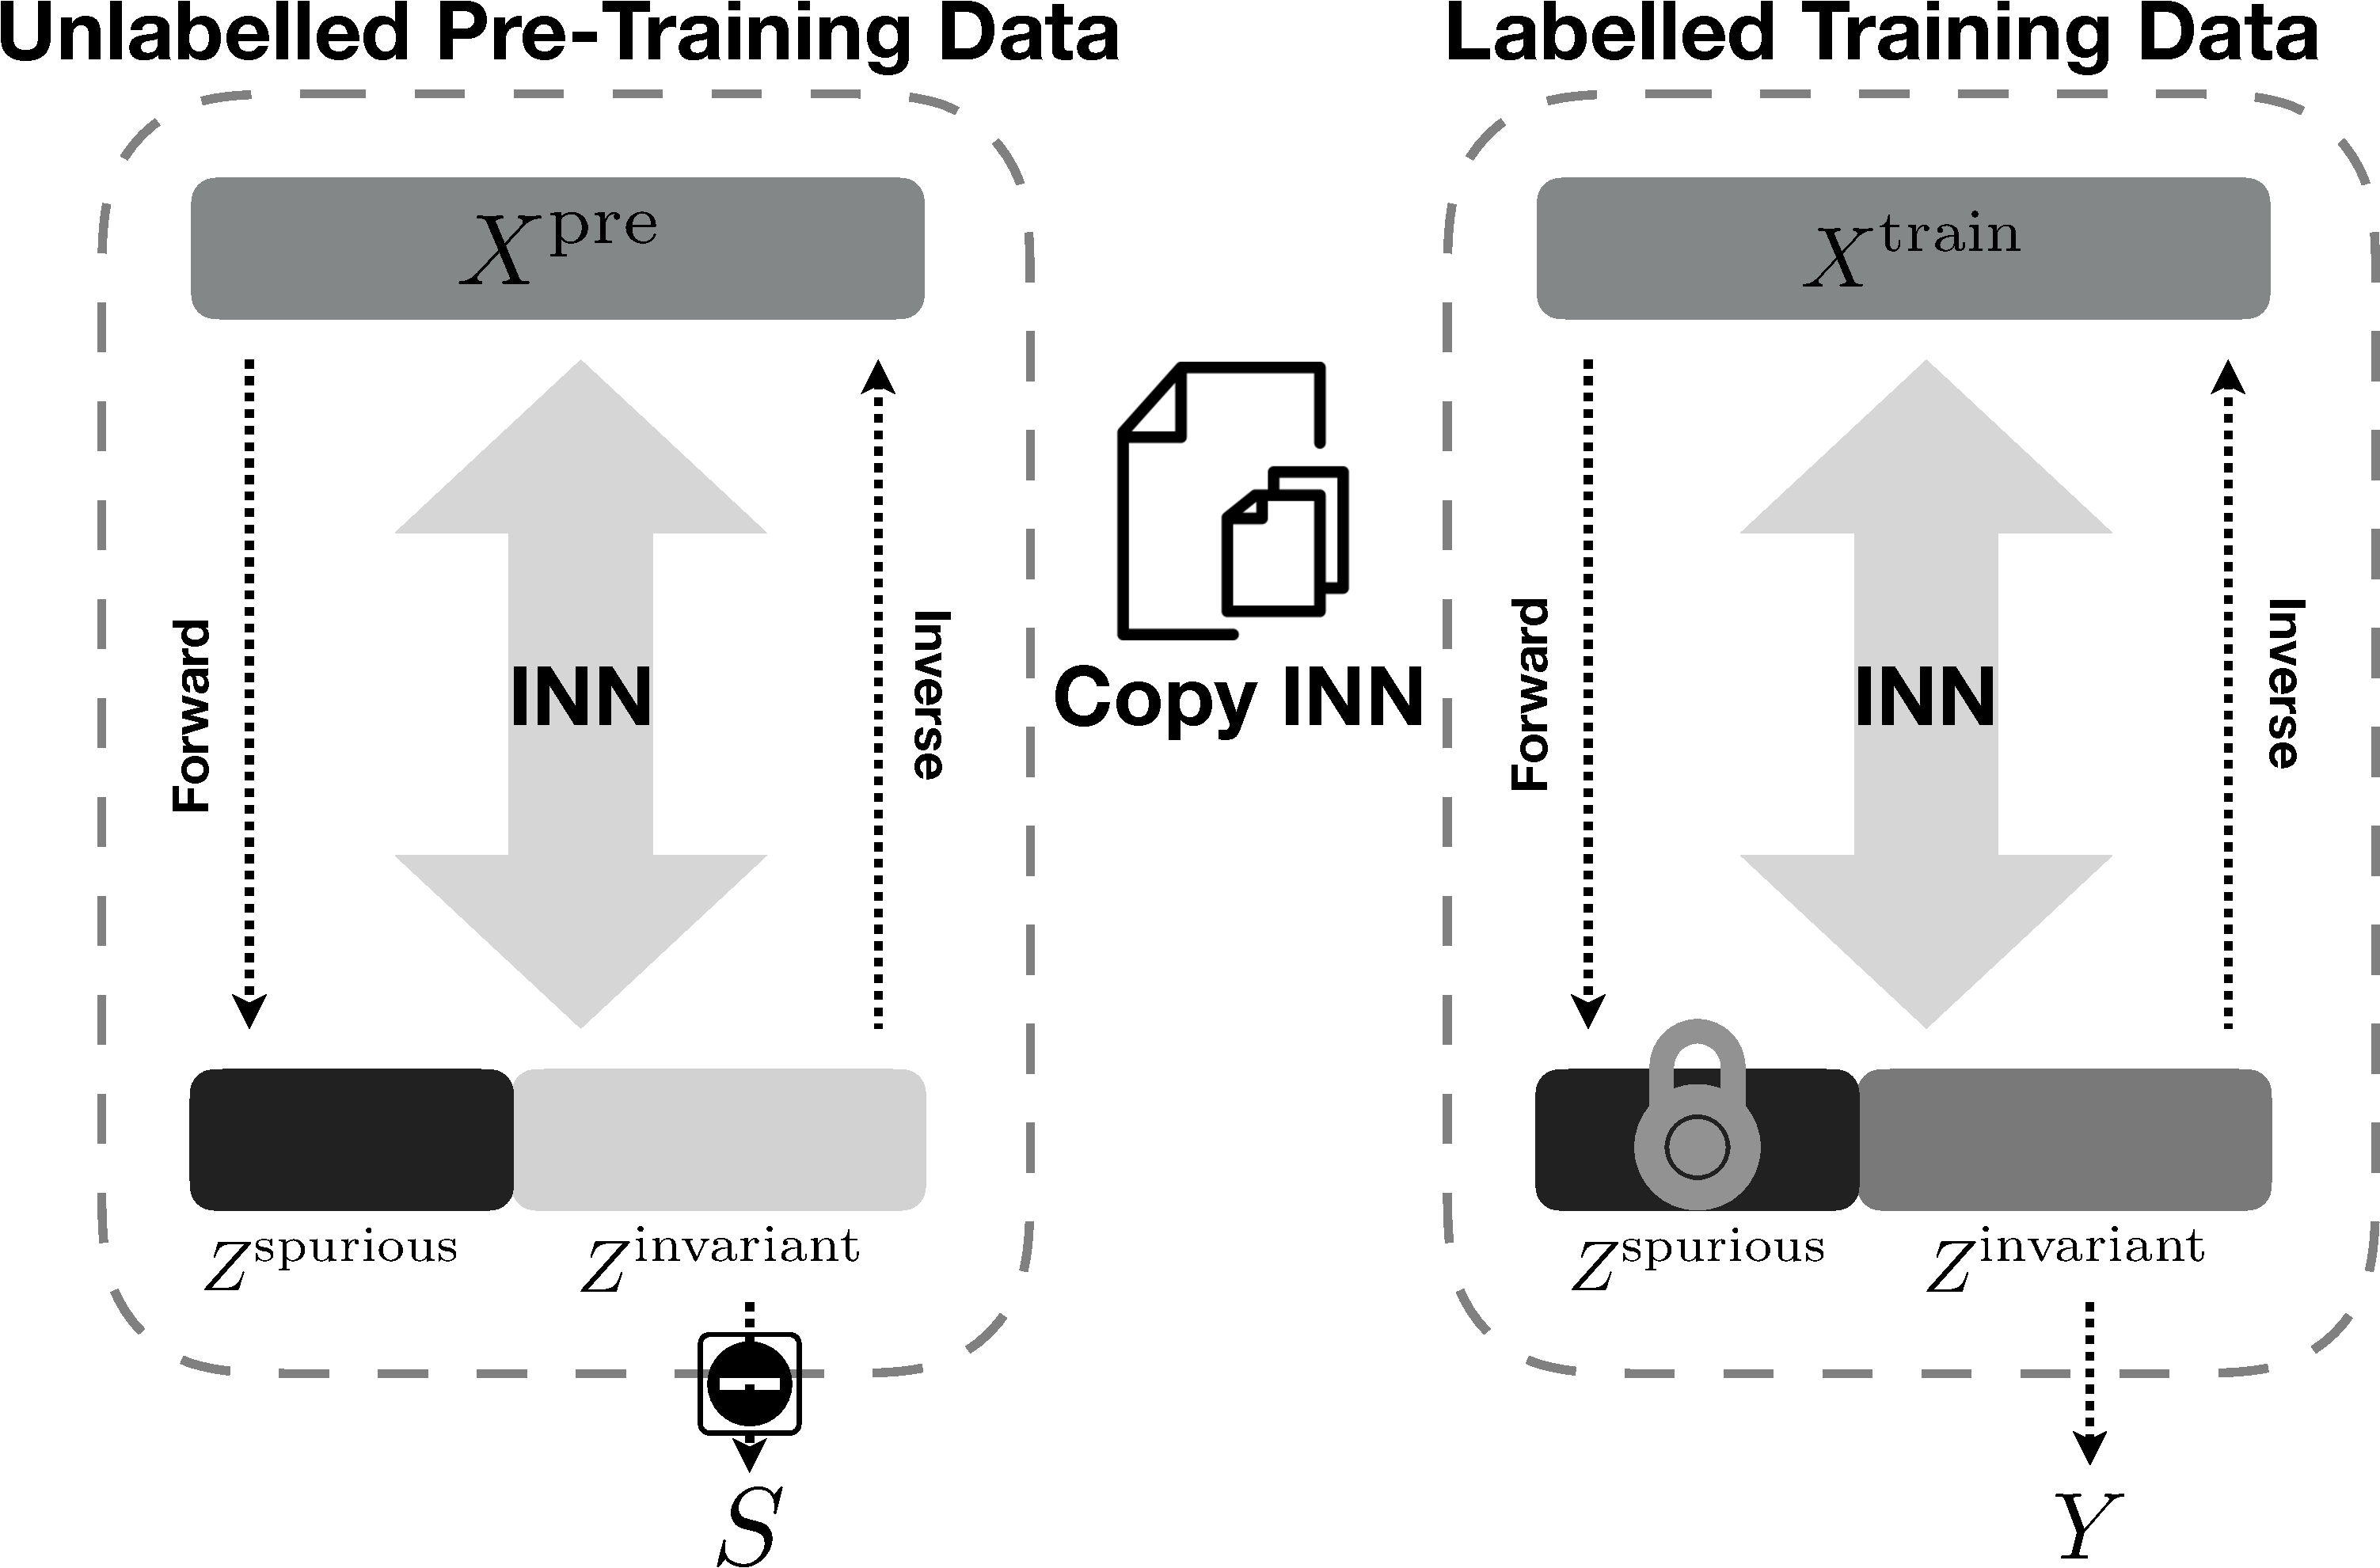
\includegraphics[width=0.4\textwidth]{./Figures/diagram.pdf}
%     \caption{Training procedure using the cFlow model for illustrative purposes.}%
%     \label{fig:training_diagram}
% \end{figure}
\begin{figure*}[tb]
    \centering
    \hfill
    \subfloat[cFlow model.]{%
        \scalebox{0.33}{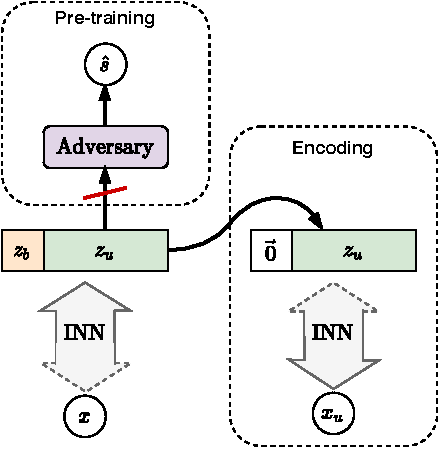
\includegraphics[width=\textwidth]{./Figures/inn_diagram_u.pdf}}%
        \label{fig:inn_diagram}
    }
    \hfill
    \subfloat[cVAE model.]{%
        \scalebox{0.4}{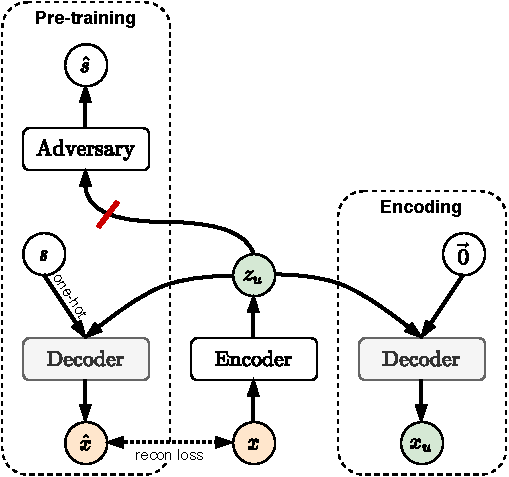
\includegraphics[width=\textwidth]{./Figures/cvae_diagram_u.pdf}}%
        \label{fig:cvae_diagram}
    }
    \hfill
    \caption{
        Training procedure for our models. $x$: input, $s$: sensitive attribute, $z_u$: de-biased representation, $x_u$: de-biased version of the input in the data domain.
        The red bar indicates a gradient reversal layer, and $\stackrel{\rightarrow}{0}$ the null-sampling operation.
    }%
    \label{fig:model-diagrams}
\end{figure*}

\subsection{Problem Statement} % HEADING IS JUST TO HELP ORGANIZE THOUGHTS, WILL BE DELETED LATER
\noindent We assume we are given inputs $\bm{x} \in \mathcal{X}$ and corresponding labels $y \in \mathcal{Y}$.
Furthermore, there is some spurious variable $s \in \mathcal{S}$ associated with each input $\bm{x}$ which we do \emph{not} want to predict. 
Let $X$, $S$ and $Y$ be random variables that take on the values $\bm{x}$, $s$ and $y$, respectively.
The fact that both $y$ and $s$ are predictive of $\bm{x}$ implies that $\mathcal{I}(X;Y), \mathcal{I}(X;S) > 0$, where $\mathcal{I}(\cdot ;\cdot)$ is the mutual information.
Note, however, that the conditional entropy is non-zero: $H(S|X) \neq 0$, i.e., $S$ is not completely determined by $X$.

%The difficulty emerges in the construction of the fully-supervised training dataset in which correspondence between $S$ and $Y$ is exaggerated compared to the test set.
The difficulty of this setup emerges in the training set: there is a close correspondence between $S$ and $Y$, such that for a model that sees the data through the lens of the loss function, the two are indistinguishable.
Furthermore, we assume that this is \emph{not} the case in the test set, meaning the model cannot rely on shortcuts provided by $S$ if it is to generalise from the training set.

We call this scenario where we only have access to the labels of a biasedly-sampled subpopulation
an \emph{aggravated fairness problem}.
These are not uncommon in the real-world.
For instance, in long-feedback systems such as mortgage-approval where the demographics of the subpopulation with observed outcomes is \emph{not} representative of the subpopulation on which the model has been deployed. 
In this case, $s$ has the potential to act as a false (or \emph{spurious}) indicator of the class label and
training a model with such a dataset would limit generalisability.
Let $(X^\mathit{tr}, S^\mathit{tr}, Y^\mathit{tr})$ then be the random variables sampled for the training set
and $(X^\mathit{te}, S^\mathit{te}, Y^\mathit{te})$ be the random variables for the test set.
The training and test sets thus induce the following inequality for their mutual information:
$\mathcal{I}(S^\mathit{tr}; Y^\mathit{tr}) \gg \mathcal{I}(S^\mathit{te}; Y^\mathit{te}) \approx 0$.

% \subsection{In an Ideal World} % HEADING IS JUST TO HELP ORGANIZE THOUGHTS, WILL BE DELETED LATER
Our goal is to learn a representation $\bm{z}_u$ that is independent of $s$ and transferable between downstream tasks.
Complementary to $\bm{z}_u$, we refer to some abstract component of the model that absorbs the unwanted information related to $s$ as $\mathcal{B}$, the realisation of which we define with respect to each of the two models to be described.
%To satisfy this objective, we introduce an additional regularisation term
%that can be viewed from an information-theoretic perspective as minimising the mutual information between the random variables:
The requirement for $\bm{z}_u$ can be expressed via mutual information:
\begin{align}
  I(\bm{z}_u;s) \overset{!}{=} 0~.
  \label{eq:migoal}
\end{align}
However, for the representation to be useful, we need to capture as much relevant information in the data as possible.
Thus, the combined objective function:
\begin{align}
  \min_{\theta} \mathbb{E}_{x \sim X}[-\log p_\theta(\bm{x})] + \lambda I(f_\theta(x);s)
  \label{eq:objectivetheory}
\end{align}
where $\theta$ refers to the trainable parameters of our model $f_\theta$ and $p_\theta(\bm{x})$ is the likelihood it assigns to the data.

We optimise this loss in an adversarial fashion by playing a min-max game, in which our encoder acts as the generative component.
The adversary is an auxiliary classifier $g$, which receives $\bm{z}_u$ as input and attempts to predict the spurious variable $s$.
We denote the parameters of the adversary as $\phi$;
for the parameters of the encoder we use $\theta$, as before.
The objective from~\eqref{eq:objectivetheory} is then% realised as
\begin{align}
  \min_{\theta\in\Theta} \max_{\phi\in\Phi} \mathbb{E}_{x \sim X}[\log p_\theta(x) -\lambda\mathcal{L}_c(g_\phi(f_\theta(x))); s)]
  \label{eq:objectivepractical}
\end{align}
where $\mathcal{L}_c$ is the cross-entropy between the predictions for $s$ and the provided labels.
In practice, this adversarial term is realised with a gradient reversal layer (GRL) \citep{ganin2016domain} between $\bm{z}_u$ and $g$ as is common in adversarial approaches~\citep{edwards2016censoring}.
% to fair representation learning

\subsection{The Disentanglement Dilemma} % HEADING IS JUST TO HELP ORGANIZE THOUGHTS, WILL BE DELETED LATER
The objective in~\eqref{eq:objectivepractical} balances the two desiderata: predicting $y$ and being invariant to $s$.
However, in the training set $(X^\mathit{tr}, S^\mathit{tr}, Y^\mathit{tr})$,
$y$ and $s$ are so strongly correlated that removing information about $s$ inevitably removes information about $y$.
This strong correlation makes existing methods fail under this setting.
% However, this objective is complicated by the desideratum that $\bm{z}_u$ remain predictive of $y$,
% which precludes us from directly training on the target-labelled dataset $(X^\mathit{tr}, S^\mathit{tr}, Y^\mathit{tr})$,
%where $y$ and $s$ are so strongly correlated that removing information about $s$ inevitably removes information about $y$.
%We therefore need
In order to even define the right learning goal,
we require another source of information that allows us to disentangle $s$ and $y$.
For this, we assume the existence of another set of samples that follow a similar distribution to the test set,
but whilst the sensitive attribute is available, the class labels are not.
In reality, this is not an unreasonable assumption,
as, while properly annotated data is scarce, unlabelled data can be obtained in abundance (with demographic information from census data, electoral rolls, etc.).
Previous work has also considered treated ``unlabelled data'' as still having $s$ labels~\citep{wick2019unlocking}.
We are restricted only in the sense that the spurious correlations we want to sever are indicated in the features.
We call this the \emph{representative set}, consisting of $X^\mathit{rep}$ and $S^\mathit{rep}$.
It fulfils $\mathcal{I}(S^\mathit{rep}; Y^\mathit{rep}) \approx 0$
(or rather, it would, if the class labels $Y^\mathit{rep}$ were available).
%{\color{red} justify the existence of such a dataset}

We now summarise the training procedure; an outline for the invertible network model (cFlow) can be seen in Fig.~\ref{fig:inn_diagram}.
First, the encoder network $f$ is trained on ($X^\mathit{rep}, S^\mathit{rep}$), during the first phase.
The trained network is then used to encode the training set,
taking in $\bm{x}$ and producing the representation, $\bm{z}_u$, decorrelated from the spurious variable.
The encoded dataset can then be used to train any off-the-shelf classifier safely, with information about the spurious variable having been absorbed by some auxiliary component $\mathcal{B}$.
In the case of the conditional VAE (cVAE) model,
$\mathcal{B}$ takes the form of the decoder subnetwork, which reconstructs the data conditional on a one-hot encoding of $s$,
while for the invertible network $\mathcal{B}$ is realised as a partition of the feature map $\bm{z}$
(such that $\bm{z} = [\bm{z}_u, \bm{z}_b]$), given the bijective constraint.
Thus, the classifier cannot take the shortcut of learning $s$ and instead must learn how to predict $y$ directly.
Obtaining the $s$-invariant representations, $\bm{x}_u$, in the data domain
is simply a matter of replacing the $\mathcal{B}$ component of the decoder's input for the cVAE,
and $\bm{z}_b$ for cFlow, with a zero vector of equivalent size.
We refer to this procedure used to generate $\bm{x}_u$ as \emph{null-sampling} (here, with respect to $\bm{z}_b)$.

% This That said, we do wish to draw a distinction between null-sampling and the annihilation operation featured in .
Null-sampling resembles the \emph{annihilation} operation described in \citet{xiao2017dna}, however we note that the two serve very different roles.  Whereas the annihilation operation serves as a regulariser to prevent trivial solutions (similar to \cite{jaiswal2018unsupervised}), null-sampling is used to generate the invariant representations post-training.

\subsection{Conditional Decoding}%
\label{conddec}
\noindent We first describe a VAE-based model similar to that proposed in~\citet{madras2018learning}, before highlighting some of its shortcomings that motivate the choice of an invertible representation learner.

The model takes the form of a class conditional $\beta$-VAE \citep{higgins2017beta}, in which the decoder is conditioned on the spurious attribute.
We use $\theta_{enc}, \theta_{dec} \in \theta$ to denote the parameters of the encoder and decoder sub-networks, respectively.
Concretely, the encoder component performs the mapping $x \rightarrow{\bm{z}_u}$, while $\mathcal{B}$ is instantiated as the decoder,
$\mathcal{B} \coloneqq p_{\theta_{dec}}(x|z_u, s)$, which takes in a concatenation of the learned non-spurious latent vector $\bm{z}_u$ and a one-hot encoding of the spurious label $s$ to produce a reconstruction of the input $\hat{x}$.
Conditioning on a one-hot encoding of $s$, rather than a single value, as done in \citet{madras2018learning} is the key to visualising invariant representations in the data domain.
If $\mathcal{I}(z_u; s)$ is properly minimised, the decoder can only derive its information about $s$ from the label, thereby freeing up $\bm{z}_u$ from encoding the unwanted information while still allowing for reconstruction of the input.
Thus, by feeding a zero-vector to the decoder we achieve $\hat{x} \perp s$.
The full learning objective for the cVAE is given as
\begin{align}
\begin{split}
    \mathcal{L}_{\mathrm{cVAE}} =& \mathbb{E}_{q_{\theta_{enc}}(z_u, b|x)}[\log p_{\theta_{dec}}(x|z, b) - \log p_{\theta_{dec}}(s|z_u)] \\ 
    &- \beta D_{KL}(q_{\theta_{enc}}(z_u |x) \| p(z_u))
\end{split}
\end{align}
where $\beta$ is a hyperparameter that determines the trade-off between reconstruction accuracy and independence constraints,
and $p(\bm{z}_u)$ is the prior imposed on the variational posterior.
For all our experiments, $p(\bm{z}_u)$ is realised as an Isotropic Gaussian.
Fig.~\ref{fig:cvae_diagram} summarises the procedure as a diagram.

While we show this setup can indeed work for simple problems, as~\citet{madras2018learning} before us have, we show that it lacks scalability due to disagreement between the components of the loss.
Since information about $s$ is only available to the decoder as a binary encoding,
if the relationship between $s$ and $x$ is highly non-linear and cannot be summarised by a simple on/off mechanism, as is the case if $s$ is an attribute such as gender,
off-loading information to the decoder by conditioning is no longer possible. As a result, $\bm{z}_u$ is forced to carry information about $s$ in order to minimise the reconstruction error. 

The obvious solution to this is to allow the encoder to store information about $s$ in a partition of the latent space as in  \citet{creager2019flexibly}.  However, we question whether an autoencoder is the best choice for this setup, with the view that an invertible model is the better tool for the task. Using an invertible model has several guarantees, namely complete information-preservation and freedom from a reconstruction loss, the importance of which we elaborate on below.

\subsection{Conditional Flow}\label{cflow}
\paragraph{Invertible Neural Networks.}
Invertible neural networks are a class of neural network architecture characterised by a bijective mapping between their inputs and output \citep{Dinh2014}. The transformations are designed such that their inverses and Jacobians are efficiently computable.
These flow-based models permit \emph{exact} likelihood estimation \citep{normflows2015} through the warping of a base density with a series of invertible transformations and computing the resulting, highly multi-modal, but still normalised, density, using the change of variable theorem:
% Flow-GAN \cite{grover2018flowgan} combines the \emph{exact} log-likelihood estimation of the invertible network with the adversarial training of a GAN.
\begin{align}
\begin{split}
  \log p(x) &= \log p(z) + 
   \sum \log \left| \det\left( \frac{\diff h_i}{ h_{i-1}}\right) \right|, %\\
  \quad p(z) = \mathcal{N}(z; 0, \mathbb{I})
  \label{eq:changeofvariables}
\end{split}
\end{align}
where $h_i$ refers to the outputs of the layers of the network and $p(z)$ is the base density, specifically an Isotropic Gaussian in our case.
Training of the invertible neural network is then reduced to maximising $\log p(x)$ over the training set,
i.e.\ maximising the probability the network assigns to samples in the training set.

% The requirement of analytic invertibility and Jacobians demands the use of a specialised subset of neural network layers, but the repertoire of practical invertible transformations has grown steadily over recent years, of which describe only the few we draw upon.

% \paragraph{Coupling layers}. Dinh et al. \cite{Dinh2014} introduced a simple yet powerful invertible transformation in the form of coupling layers. Ease of invertibility is achieved by updating only half of the input vector with a function that itself is trivially invertible but that is at the same time parameterised by a arbitrarily complex operation not subject to the invertibility constraint (e.g. a multi-layer neural network).
% Concretely, the vector $\bm{u}$ is split into two evenly sized vectors: $\bm{u} = [\bm{u}_1, \bm{u}_2]$.
% The output of the coupling layer is then a concatenation of vectors $\bm{v}_1$ and $\bm{v}_2$,
% where $\bm{v}_1 = s \cdot \bm{u}_1 + t$ and $\bm{v}_2 = \bm{u}_2$, with the affine parameters $s$ and $t$ generated by a non-invertible function of $\bm{u}_2$.

% \paragraph{1x1 Convolutions}. Kingma and Dhariwal \cite{KinDha18} introduced invertible 1x1 convolution as a generalised permutation operation and show that determinant can be computed efficiently using an LU decomposition of the weights.

% \paragraph{Spatial downsampling.} To downsample the spatial dimensions and promote mixing between the variables, \cite{Dinh2014} first mask the input with a checkerboard pattern before reshaping (transforming a $c \times h\times w$ tensor into a $4c \times \frac{1}{2} h\times \frac{1}{2}w$). Each "level" of the network is demarcated by a downsampling operation.

\paragraph{The Benefits of Bijectivity.}
Using an invertible network to generate our encoding, $\bm{z}_u$, carries a number of advantages over other approaches.
Ordinarily, the main benefit of flow-based models is that they permit exact density estimation. 
However, since we are not interested in sampling from the model's distribution, in our case the likelihood term serves as a regulariser, as it does for  \citet{JacSmeOya18}. 
Critically, this forces the mean of each latent dimension to zero enabling null-sampling. 
The invertible property of the network guarantees the preservation of all information relevant to $y$ which is independent of $s$, regardless of how it is allocated in the output space.
Secondly, we conjecture that the encodings are more robust to out-of-distribution data.
Whereas an autoencoder could map a previously seen input and a previously unseen input to the same representation,
an invertible network sidesteps this due to the network's bijective property, ensuring all relevant information is stored somewhere. This opens up the possibility of transfer learning between datasets with a similar manifestation of $s$, as we demonstrate in the Appendix~\ref{sec:transfer-learning}.

Under our framework, the invertible network $f$ maps the inputs $\bm{x}$ to a representation $\bm{z}_u$:
$f(\bm{x}) = \bm{z}$.
We interpret the embedding $\bm{z}$ as being the concatenation of two smaller embeddings: $\bm{z} = [\bm{z}_u, \bm{z}_b]$.
The dimensionality of $\bm{z}_b$, and $\bm{z}_u$, by complement, is a free parameter (see section~\ref{sec:optimisation-details} for tuning strategies).
As $f$ is invertible, $\bm{x}$ can be recovered like so:
\begin{align}
  \bm{x} = f^{-1}([\bm{z}_u, \bm{z}_b])
  \label{eq:zreconstruct}
\end{align}
where $\bm{z}_b$ is required for equality of the output dimension and input dimension to satisfy the bijectivity of the network -- we cannot output $\bm{z}_u$ alone, but have to output $\bm{z}_b$ as well. In order to generate the pre-image of $\bm{z}_u$, we perform null-sampling with respect to $\bm{z}_b$ by zeroing-out the elements of $\bm{z}_b$ (such that $\bm{x}_{u} = f^{-1}([\bm{z}_{u}, \stackrel{\rightarrow}{0}])$), i.e. setting them to the mean of the prior density, $\mathcal{N}(z;0, I)$.

How can we be sure that $\bm{z}_u$ contains enough information about $y$?
The importance of the invertible architecture bears out from this consideration. %, as the bijectivity of the network guarantees preservation of all information about the input. %
% The existence of the inverse, $f^{-1}$,  p $x$ from $z$ because $f^{-1}$ exists and can do just that.
As long as $\bm{z}_b$ does not contain the information about $y$, $\bm{z}_u$ necessarily must.
We can raise or lower the information capacity of $\bm{z}_b$ by adjusting its size;
this should be set to the smallest size sufficient to capture all information about $s$, so as not to sacrifice class-relevant information.
Section~\ref{sec:additional-results} explores the effects of the size further.

% Eq~\eqref{eq:zreconstruct} defines how to obtain $\bm{x}$.
% In order to generate the pre-image of $\bm{z}_u$, we perform null-sampling with respect to $\bm{z}_b$ by zeroing-out its elements -- i.e. setting them to the mean of the prior density imposed on $\bm{z}$, $\mathcal{N}(z;0, I)$ -- by the operation, $\bm{x}_{u} = f^{-1}([\bm{z}_{u}, \stackrel{\rightarrow}{0}])$.

% \paragraph{Tuning the Partition Sizes.}

% \paragraph{The Pitfalls of Adversarial Training.}

% \paragraph{Preprocessing}.
% Heuristically, we found that preprocessing the data with an autoencoder stabilises and accelerates training of the cFlow model. The autoencoder was pretrained on the pretraining set solely to minimise reconstruction loss and its weights frozen at the time of the INN's training. While this means the INN is not truly lossless with respect to the uncompressed data, its bijectivity is leveraged to ensure semantically-relevant information is not discarded during the pre-training phase, which is still applicable since the autoencoder is not trained jointly with the INN to maximise the adversarial loss. Since the autoencoder is optimised for compression, information about both the spurious and non-spurious attributes is captured impartially in its encoding.

%%%%%%%%% Experiments

\section{Experiments}
\noindent We present experiments to demonstrate that the null-sampled representations are in fact invariant to $s$
while still allowing a classifier to predict $y$ from them.
We run our cVAE and cFlow models on the coloured MNIST (cMNIST) and CelebA dataset,
which we artificially bias, first describing the sampling procedure we follow to do so for non-synthetic datasets.
As baselines we have the model of~\citet{kim2019learning} (Ln2L) and the same CNN used to evaluate the cFlow and cVAE models
but with the unmodified images as input (CNN).
For the cFlow model we adopt a Glow-like architecture~\citep{KinDha18},
while both subnetworks of the cVAE model comprise gated convolutions~\citep{van2016conditional}, where the encoding size is $256$.
For cMNIST, we construct the Ln2L baseline according to its original description, for CelebA,
we treat it as an augmentation of the baseline CNN's objective function.
%More
Detailed information regarding model architectures can be found in sections~\ref{sec:architectures} and~\ref{sec:optimisation-details}.%
\footnote{The code can be found at \url{https://github.com/predictive-analytics-lab/nifr}.}
% \begin{figure*}[!htb]
%   \centering
%   %
%   \subfloat[CelebA]{\scalebox{0.495}{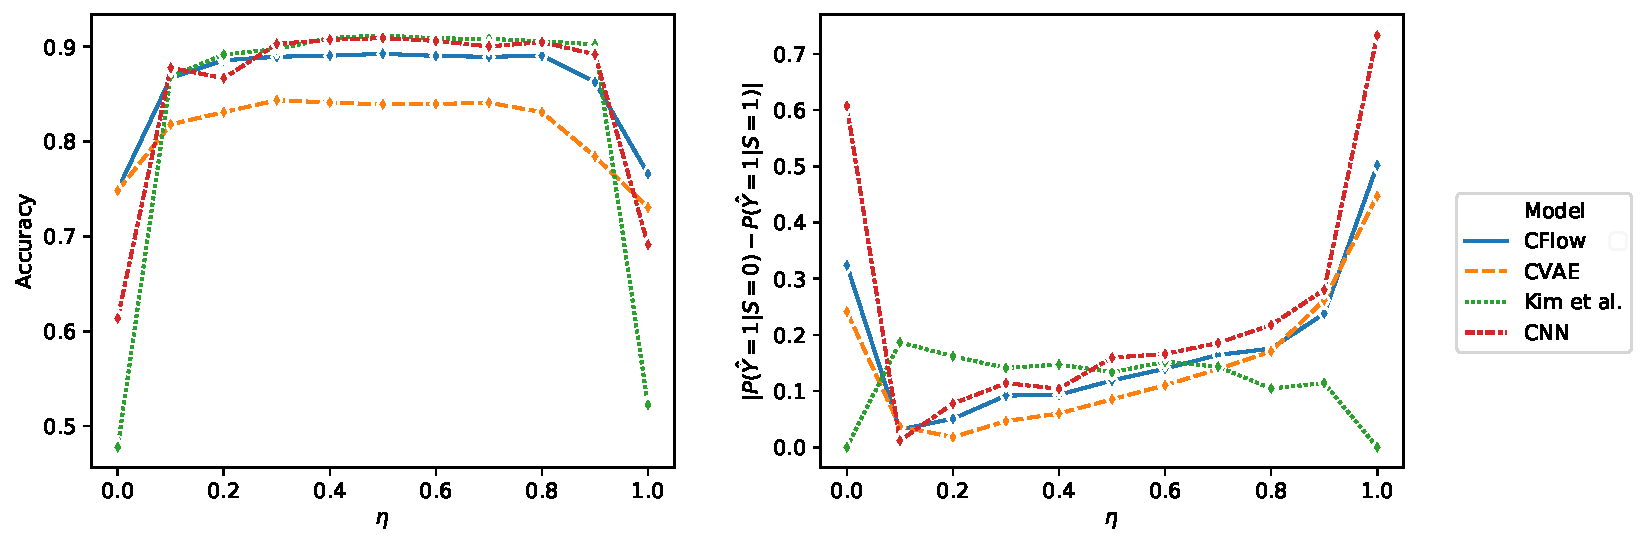
\includegraphics[width=\textwidth]{./results/celeba/celeba_acc_DP.pdf}}
%   \label{fig:celeba_chart}
%   }%
%   %\hfill
%   \subfloat[UCI Adult]{\scalebox{0.495}{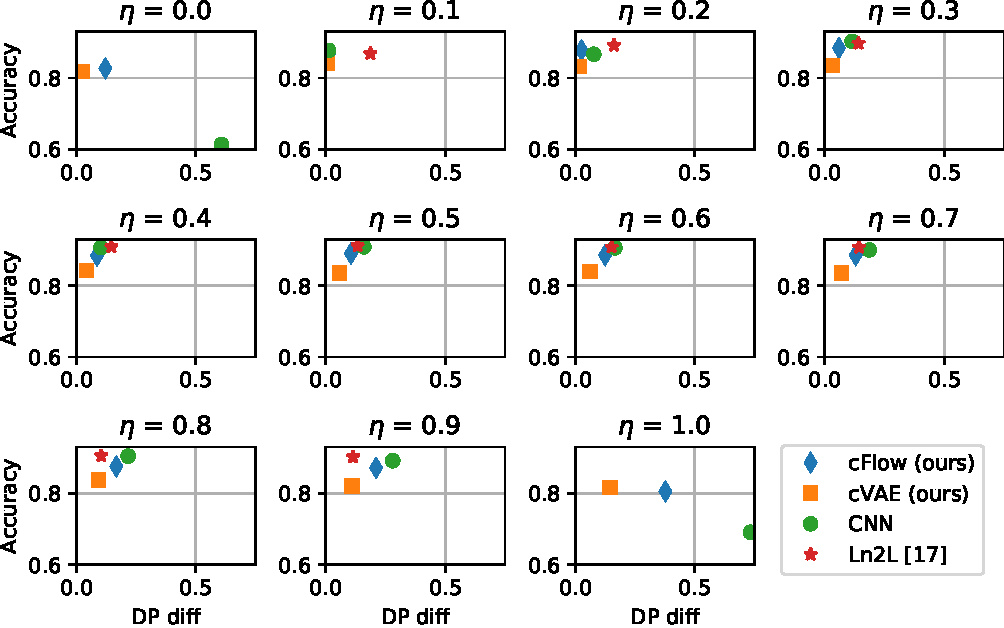
\includegraphics[width=\textwidth]{paper2/Figures/nosinn_celeba_multiplot_all_landscape_Smiling.pdf}}
%   \label{fig:adult_chart}
%   }%
%   \caption{
%     Performance of our approach on the CelebA and UCI Adult datasets.
%     (Left of each) We show the accuracy of a downstream classifier trained on representations learned by our model.
%     (Right of each) We show the Demographic Parity of a model trained on our representations (the lower the better).
%   }\label{fig:chart}
% \end{figure*}
\begin{figure}[tb]
    \centering
    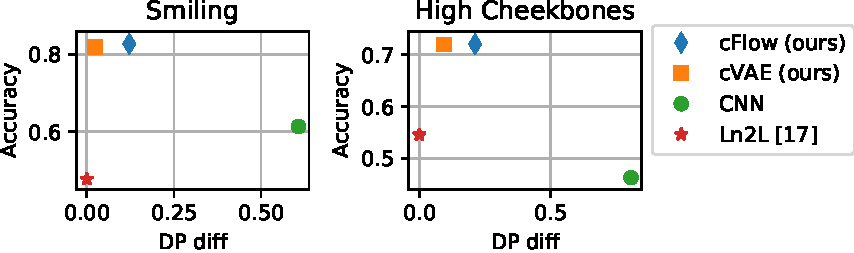
\includegraphics[width=0.7\textwidth]{paper2/Figures/nosinn_celeba.pdf}
    \caption{
        Performance of our model for different targets (mixing factor $\eta=0$).
        Left: \emph{Smiling} as target, right: \emph{high cheekbones}.
        \emph{DP diff} measures fairness with respect to demographic parity.
        A perfectly fair model has a \emph{DP diff} of 0.
    }%
    \label{fig:celeba-targets}
\end{figure}

\begin{figure}[tb]
    \centering
    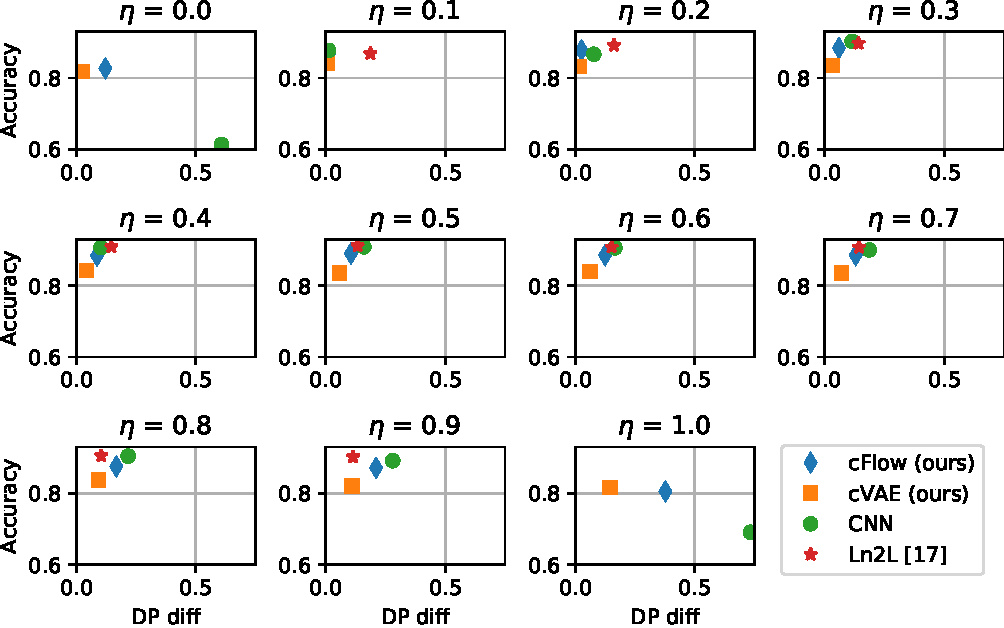
\includegraphics[width=0.85\textwidth]{paper2/Figures/nosinn_celeba_multiplot_all_landscape_Smiling.pdf}
    \caption{
        Performance of our model for the target ``smiling'' for different mixing factors $\eta$.
        \emph{DP diff} measures fairness with respect to demographic parity.
        A perfectly fair model has a \emph{DP diff} of 0, thus the closer to top-left the better it is in terms of we accuracy-fairness trade-off.
        Only values $\eta=0$ and $\eta=1$ correspond to the scenario of a strongly biased training set.
        The results for $0.1\leq \eta\leq 0.9$ are to confirm that our model does not harm performance for non-biased training sets.
    }%
    \label{fig:celeba-multiplot}
\end{figure}

% \begin{figure*}[!htb]
%   \centering
%   \caption{Performance of our methods (cVAE and cFlow) on the tabular UCI Adult Dataset. This is a common benchmark in fair machine learning literature. Each model depicts the result of a ownstream classifier trained on the embeddings produced by one of the models. (Left) Accuracy of a downstream classifier. (Middle) Demographic Parity of a downstream classifier. (Right) Equality of Opportunity of a downstream classifier.}\label{fig:adult_results}
% \end{figure*}
\subsection{Synthesising Dataset Bias}
For our experiments, we require a training set that exhibits a strong spurious correlation, together with a test set that does not.
For cMNIST, this is easily satisfied as we have complete control over the data generation process.
For CelebA and  UCI Adult, on the other hand,
we have to generate the split from the existing data.
To this end, we first set aside a randomly selected portion of the dataset from which to sample the biased dataset
The portion itself is then split further into two parts:
one in which $(s=-1 \land y=-1) \lor (s=+1 \land y=+1)$ holds true for all samples, call this part $\mathcal{D}_{eq}$,
and the other part, call it $\mathcal{D}_{opp}$, which contains the remaining samples.
To investigate the behaviour at different levels of correlation,
we mix these two subsets according to a mixing factor $\eta$.
For $\eta \leq \tfrac{1}{2}$, we combine (all of) $\mathcal{D}_{eq}$
with a fraction of $2\eta$ from $\mathcal{D}_{opp}$.
For $\eta > \tfrac{1}{2}$, we combine (all of) $\mathcal{D}_{opp}$
and a fraction of $2(1 -\eta)$ from $\mathcal{D}_{eq}$.
Thus, for $\eta=0$, the biased dataset is just $\mathcal{D}_{eq}$,
for $\eta=1$ it is just $\mathcal{D}_{opp}$
and for $\eta=\tfrac{1}{2}$ the biased dataset is an ordinary subset of the whole data. The test set is simply the data remaining from the initial split.

\subsection{Evaluation protocol}
We evaluate our results in terms of accuracy and fairness.
A model that perfectly decouples its predictions from $s$ will achieve near-uniform accuracy across all biasing-levels.
For binary $s$/$y$ we quantify the fairness of a classifier's predictions using \emph{demographic parity} (DP): the  absolute difference in the probability  of a positive prediction for each sensitive group.

% We also calculate the absolute difference in Equality of Opportunity \cite{hardt2016equality}, which is the relationship between True Positive Rates of subgroups with the same sensitive attribute.

\begin{figure}[tb]
    \centering
    % 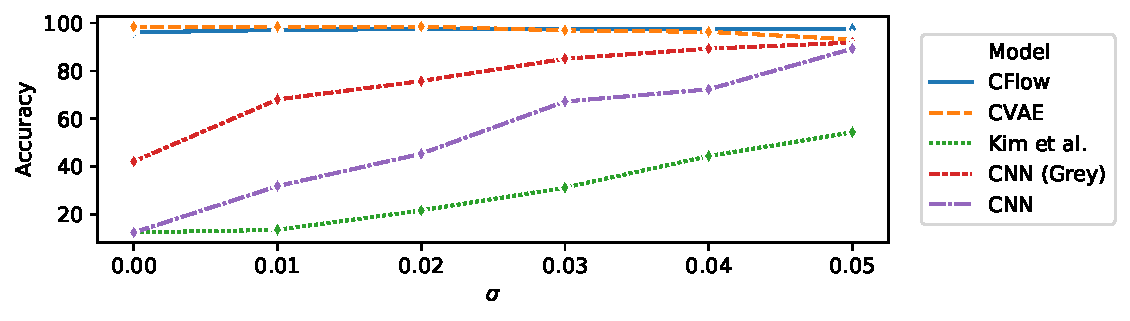
\includegraphics[width=0.9\textwidth]{./results/cmnist/cmnist_results.pdf}
    % 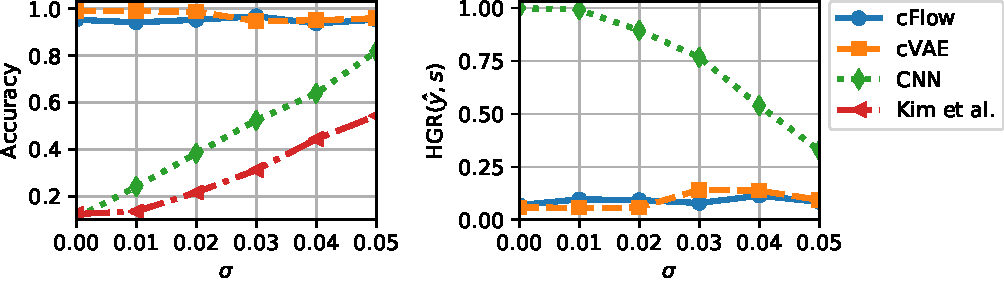
\includegraphics[width=0.9\textwidth]{paper2/Figures/cmnist_new.pdf}
    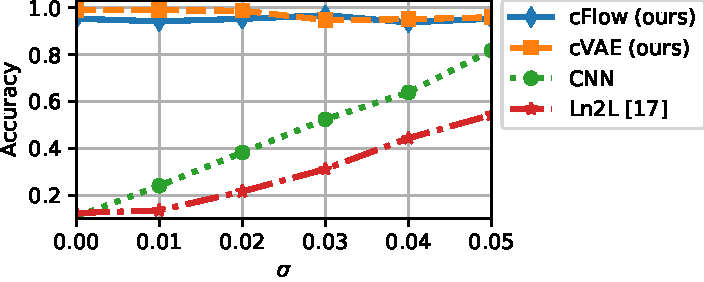
\includegraphics[width=0.7\textwidth]{paper2/Figures/cmnist_new_no_hgr.pdf}
    \caption{
        % Accuracy and correlation (HGR) of predictions $\hat{y}$ and $s$ of our approach in comparison with other baseline models on the cMNIST dataset, for different standard deviations ($\sigma$) for the colour sampling.
        Accuracy of our approach in comparison with other baseline models on the cMNIST dataset, for different standard deviations ($\sigma$) for the colour sampling.
    }%
    \label{fig:cmnist_chart}
\end{figure}
\subsection{Experimental results}
% \noindent Our model can be applied to tabular data and image data alike.
% Due to space constraints, the experiments with the tabular dataset \emph{UCI Adult} are situated in the Appendix.
%To illustrate the effectiveness and generality of our framework, we apply our models to a tabular dataset, in the UCI Adult dataset,
We report the results from two image datasets.
cMNIST, a synthetic dataset, is a good starting point for evaluating our model due to the direct control we have over the biasing.
CelebA, on the other hand, is a more practical and challenging example.
% To illustrate the generality of our approach,
We also test our method on a tabular dataset, the Adult dataset.
%For full details regarding the architectures of our models and their optimisation, see the Appendix.

\paragraph{cMNIST.}
The coloured MNIST (cMNIST) dataset is a variant of the MNIST dataset in which the digits are coloured.
In the training set, the colours have a one-to-one correspondence with the digit class.
In the test set (and the representative set), colours are assigned randomly.
The colours are drawn from Gaussians with 10 different means.
We follow the colourisation procedure outlined by~\citet{kim2019learning}, with the mean colour values selected so as to be maximally dispersed.
The full list of such values can be found in section~\ref{sec:color-details}.
We produce multiple variants of the cMNIST dataset corresponding to different standard deviations $\sigma$ for the colour sampling:
$\sigma \in \{0.00, 0.01, ..., 0.05 \}$.
% The images are symmetrically zero-padded to a size of $32 \times 32$ to allow for an additional downsampling stage in the cFlow model.
% No additional data augmentation is used.
% 24,000 of the 36,000 training samples were set aside for representative, the remaining 10,000 for training the downstream classifier.
% We continue to use 10,000 samples usually reserved for testing on vanilla MNIST for that same purpose.

For this specific dataset, we can establish an additional baseline by simply grey-scaling the dataset
% Since the data-generation process is known, we can establish a baseline an additional by following the simple heuristic of grey-scaling the dataset
which only leaves the luminosity as spurious information.
%The grey-scaling operation does not completely eliminate the bias in the dataset, it only mitigates it by reducing the number of unique values for $s$ it is still exhibited residually in the luminosity of the digits.
We also evaluate the model, with all the associated hyperparameters, from~\citet{kim2019learning}.
The only difference between the setups is the dataset creation, including the range of $\sigma$ values we consider.
Our versions of the dataset, on the whole, exhibit much stronger colour bias, to the point of the mapping the digit's colour and class being bijective.
Fig.~\ref{fig:cmnist_chart} shows that the model significantly underperforms even the na\"ive baseline, aside from at $\sigma = 0$, where they are on par.

Inspection of the null-samples shows that both the cVAE and cFlow model succeed in removing almost all colour information, which is supported quantitatively by fig.~\ref{fig:cmnist_chart}.
While the cVAE outperforms cFlow marginally at low $\sigma$ values, performance degrades
%rapidly
as this increases.
This highlights the problems with the conditional decoder we anticipated in section~\ref{conddec}.
The lower $\sigma$, and therefore the variation in sampled colour, is, the more reliably the $s$ label, corresponding to the mean of RGB distribution, encodes information about the colour.
For higher $\sigma$ values, the sampled colours can deviate far from the mean and so the encoder must incorporate information about $s$ into its representation if it is to minimise the reconstruction loss.
cFlow, on the other hand, is consistent across $\sigma$ values.

\paragraph{CelebA.}
To evaluate the effectiveness of our framework on real-world image data we use the CelebA dataset~\citep{liu2015faceattributes}, consisting of 202,599 celebrity images.
These images are annotated with various binary physical  attributes, including ``gender'', ``hair colour'', ``young'', etc, from which we  select our sensitive and target attributes.
The images are centre cropped and resized to $64\times64$, as is standard practice.
For our experiments, we designate ``gender'' as the sensitive attribute,
and ``smiling'' and ``high cheekbones'' as target attributes.
We chose gender as the sensitive attribute as it a common sensitive attribute in the fairness literature.
For the target attributes, we chose attributes that are harder to learn than gender and which do not correlate too strongly with gender in the dataset
(``wearing lipstick'' for example being an attribute too closely correlated with gender).
% The sampling and evaluation procedure is identical to that conducted for the UCI Adult dataset.
% We evaluate the performance of all models for mixing factors ($\eta$) of value $\{0, 0.1, ..., 1\}$. 
The model is trained on the representative set (normal subset of CelebA)
and is then used to encode the artificially biased training set and the test set.
The results for the most strongly biased training set ($\eta=0$) can be found in fig.~\ref{fig:celeba-targets}.
Our method outperforms the baselines in accuracy and fairness.

We also assess performance for different mixing factors ($\eta$) which correspond to varying degrees of bias in the training set
(see fig.~\ref{fig:celeba-multiplot}).
This is to verify that the model does not \emph{harm} performance when there is not much bias in the training set.
For these experiments, the model is trained once on the representative set and is then used to encode different training sets.
The results show that for the intermediate values of $\eta$, our model incurs a small penalty in terms of accuracy,
but at the same time makes the results \emph{fairer} (corresponding to an accuracy-fairness trade-off). Qualitative results can be found in fig.~\ref{fig:celeba_cflow} (images from cVAE can be found in section~\ref{sec:qual-results-celeba}).

To show that our method can handle multinomial, as well as binary, sensitive attributes, we also conduct experiments with $s=\textrm{hair colour}$ as a ternary attribute (``Blonde'', ``Black'', ``Brown''), excluding ``Red'' because of the paucity of samples and the noisiness of their labels. The results for these experiments can be found in section~\ref{sec:additional-results}.
% Looking at the produced invariant representations,
% The failure of the cVAE to model complex interactions between $x_u$ and $s$ is brought to bear here.
% Due to the balancing between the adversarial and reconstruction losses,
% information relevant to the downstream task of predicting ``smiling'' is lost during the pre-training phase,
% leading to poor performance at all values of $\eta$ except the most extreme ones,
% for which it does reasonably well at mitigating the sampling bias (Fig.~\ref{fig:celeba_chart}).
% Meanwhile, cFlow does not suffer this drawback -- the images remain sharp
% (see Fig.~\ref{fig:cflow_celeba_recon_y} in comparison to Fig. \ref{fig:cvae_celeba_recon_y})
% and the accuracy obtained by training on them is comparable to the baseline at intermediary values -- and at the same time matches and outperforms the cVAE at $\eta = 0$ and $\eta = 1$, respectively.
% For these same values,
% incorporating the mutual information loss proposed by~\cite{kim2019learning} into the classifier's loss function greatly harmed performance measured by accuracy;
% the DP is zero due to all predictions being negative.

% \begin{wrapfigure}{l}{0.6\linewidth}
\begin{figure}[tb]
  \centering
  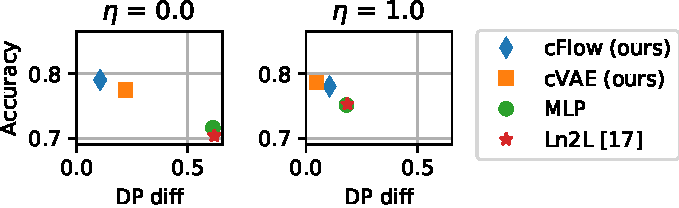
\includegraphics[width=0.6\textwidth]{paper2/Figures/nosinn_adult_multiplot_mini_diff.pdf}
  \caption{
      Results for the \textsc{Adult} dataset.
      The $x$-axis corresponds to the difference in positive rates.
      An ideal result would occupy the \textsc{top-left}.
  }%
  \label{fig:adult-chart}
\end{figure}
% \end{wrapfigure}

\paragraph{Results for the UCI Adult dataset.}
The UCI Adult dataset consists of census data and is commonly used to evaluate models focused on algorithmic fairness.
Following convention, we designate ``gender'' as the sensitive attribute $s$ and whether an individual's salary is \$50,000 or greater as $y$.
We show the performance of our approach in comparison to baseline approaches in fig. \ref{fig:adult-chart}.
We evaluate the performance of all models for mixing factors ($\eta$) $0$ and $1$. 
Results shown in fig. \ref{fig:adult-chart} show that
%while our model fails to surpass the baseline models in terms of accuracy for the balanced case (and those close to it),
we match or exceed the baseline.
%as $\eta$ moves the dataset towards a more imbalanced setting.
In terms of fairness metrics, our approach generally outperforms the baseline models for both of $\eta$.
Detailed results can be found in section~\ref{sec:additional-results}.

We also did experiments to show that the encoder transfers to other tasks. These transfer-learning experiments can be found in section~\ref{sec:transfer-learning}.


% \begin{figure}
%   \centering
%   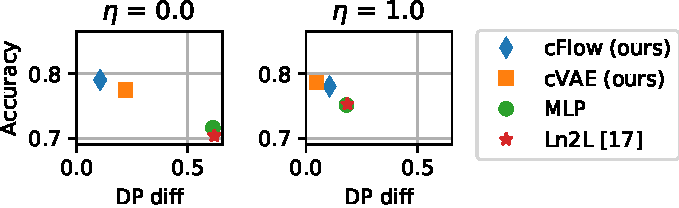
\includegraphics[width=0.7\textwidth]{paper2/Figures/nosinn_adult_multiplot_mini_diff.pdf}
%   \caption{
    %   Results for the \textsc{Adult} dataset.
    %   The $x$-axis corresponds to the difference in positive rates.
    %   An ideal result would occupy the \textsc{top-left}.
%   }%
%   \label{fig:adult-chart}
% \end{figure}

\section{Conclusion}\label{sec:conclusion}
%%%%%%%%%%%%% DISCUSSION %%%%%%%%%%%%%%%
% Controlling the correlations a computer vision and machine learning system discovers is known to be a difficult problem.
% Recent work~\cite{JoBen17,GatEckBet17,JacBehZemBet19} has shown that state-of-the-art deep convolutional neural network (CNN) systems strongly rely on \emph{shortcuts}. 
% Examples of these shortcuts include spectral statistical regularities and stationary statistics such as colours and textures. 
% Indeed, it has been shown that standard ImageNet-trained classifiers place much more weight on object textures compared to object shapes \cite{Geir18}.  As discussed in \cite{zhang2018examining} the representation flaws that result from these shortcuts can be difficult to pick up on because the test images may exhibit a similar bias.
% Those systems rely less on higher-level abstract concepts such as shape and appearance than on such details highly-correlated with, but unconnected to the classification.
% While this may be acceptable, and even desirable in certain cases (e.g. when combining image content and style from two separate images \cite{gatys2016image}), to achieve robustness, machine learning models have to look beyond \emph{spurious} correlations to those that hold true regardless of context.
% By doing so, the system can learn to produce accurate and reliable predictions, even when deployed in settings radically different from the one in which it was trained.
% However, if the training set contains spurious correlations, then a computer vision and machine learning system cannot learn the true relations just from that dataset.
% We either need to supply an inductive bias \cite{locatello2019challenging} or additional information which we can incorporate into learning.

% As a step towards solving these problems,
We have proposed a general and straightforward framework for producing invariant representations, under the assumption that a representative but partially-labelled \emph{representative} set is available.
Training consists of two stages:
an encoder is first trained on the representative set to produce a representation that is invariant to a designated spurious feature. 
This is then used as input for a downstream task-classifier, the training data for which might exhibit extreme bias with respect to that feature.
We train both a VAE- and INN-based model according to this procedure, and show that the latter is particularly well-suited to this setting due to its losslessness. 
The design of the models allows for representations that are in the data domain and therefore exhibit meaningful invariances. 
We characterise this for synthetic as well as real-world datasets for which we develop a method for simulating sampling bias.

\section*{Acknowledgements}
This work was in part funded by the European Research Council 
under the ERC grant agreement no. 851538.
We are grateful to NVIDIA for donating GPUs.

% updated April 2002 by Antje Endemann
% Based on CVPR 07 and LNCS, with modifications by DAF, AZ and elle, 2008 and AA, 2010, and CC, 2011; TT, 2014; AAS, 2016; AAS, 2020

% \documentclass[runningheads]{llncs}
% \usepackage{graphicx}
% \usepackage{comment}
% \usepackage{amsmath,amssymb,amsfonts,bm} % define this before the line numbering.
% \usepackage{color}
% \usepackage{tabularx}
% \usepackage{appendix}

% % our packages
% \usepackage{import}
% % \usepackage{subcaption}
% \usepackage[caption=false]{subfig}
% \usepackage{mathtools}
% \usepackage{booktabs}

% INITIAL SUBMISSION - The following two lines are NOT commented
% CAMERA READY - Comment OUT the following two lines
% \usepackage{ruler}
% \usepackage[width=122mm,left=12mm,paperwidth=146mm,height=193mm,top=12mm,paperheight=217mm]{geometry}

% Macros
% \def\ci{\perp\!\!\!\perp}
% \newcommand*\diff{\mathop{}\!\mathrm{d}}
% \def\httilde{\mbox{\tt\raisebox{-.5ex}{\symbol{126}}}}


% \begin{document}
% \renewcommand\thelinenumber{\color[rgb]{0.2,0.5,0.8}\normalfont\sffamily\scriptsize\arabic{linenumber}\color[rgb]{0,0,0}}
% \renewcommand\makeLineNumber {\hss\thelinenumber\ \hspace{6mm} \rlap{\hskip\textwidth\ \hspace{6.5mm}\thelinenumber}}
% \linenumbers
% \pagestyle{headings}
% \mainmatter
% \def\ECCVSubNumber{5488}  % Insert your submission number here

% \title{Null-sampling for Interpretable and \\Fair Representations -- Appendix} % Replace with your title

% % INITIAL SUBMISSION 
% \begin{comment}
% \titlerunning{ECCV-20 submission ID \ECCVSubNumber} 
% \authorrunning{ECCV-20 submission ID \ECCVSubNumber} 
% \author{Anonymous ECCV submission}
% \institute{Paper ID \ECCVSubNumber}
% \end{comment}
% %******************

% % CAMERA READY SUBMISSION
% %\begin{comment}
% \titlerunning{Appendix}
% % If the paper title is too long for the running head, you can set
% % an abbreviated paper title here
% %
% \author{Thomas Kehrenberg \and
% Myles Bartlett \and
% Oliver Thomas \and \\
% Novi Quadrianto}
% %
% \authorrunning{T. Kehrenberg et al.}
% % First names are abbreviated in the running head.
% % If there are more than two authors, 'et al.' is used.
% %
% \institute{Predictive Analytics Lab (PAL), University of Sussex, Brighton, UK
% \email{\{t.kehrenberg,m.bartlett,ot44,n.quadrianto\}@sussex.ac.uk}}
% %\end{comment}
% %******************

% \title{Appendix}
% \author{}
% \institute{}
% \maketitle
% \thispagestyle{headings}

\section{Appendix}\label{sec:nifr-appendix}

% \begin{appendix}

\subsection{Model Architectures}%
\label{sec:architectures}
\noindent For both cMNIST and CelebA we parameterise the coupling layers with the same convolutional architecture as in \citet{KinDha18}, consisting of $3$ convolutional layers each with $512$ filters of, in order, sizes $3\times3$, $1\times1$, and $3\times3$.
Following \citet{ardizzone2019guided}, we Xavier initialise all but the last convolutional layer of the $s$ and $t$ sub-networks which itself is zero-initialised so that the coupling layers begin by performing an identity transform. We used a Glow-like architecture \citep{KinDha18} (affine coupling layers together with checkerboard reshaping and invertible $1\times1$ convolutions) for the convolutional INNs. Table \ref{tab:inn_architectures} summarises the INN architectures used for each dataset.

For the image datasets each level of the cVAE encoder consists of two gated convolutional layers \citep{van2016conditional} with ReLU activation. 
At each subsequent level, the number of filters is doubled, starting with an initial value 32 and 64 in the case of CelebA and cMNIST respectively. 
In the case of the Adult dataset, we use an encoder with one fully-connected hidden layer of width $35$, followed by SeLU activation \citep{klambauer2017self}. 
For both cMNIST and CelebA, we downsample to a feature map with spatial dimensions $8\times8$, but with $3$ and $16$ channels respectively. 
For the Adult dataset, the encoding is a vector of size $35$. 
The output layer specifies both the parameters (mean and variance) of the representation's distribution. 
In all cases the KL-divergence is computed with respect to a standard isotropic Gaussian prior. 
Details of the encoder architectures can be found in table \ref{tab:vae_architectures}. The loss pre-factors were sampled from a logarithmic scale; without proper balancing the networks can exhibit instability, especially during the early stages of training.

\begin{table}[tp]
\caption{INN architecture used for each dataset.}
\label{tab:inn_architectures}
\centering
\begin{tabular}{lllll}
\toprule
Dataset & Levels & Level depth & Coupl. chan. & Input to discr. \\ \midrule
UCI Adult                   & 1      & 1     & 35       & Null-samples       \\
cMNIST                      & 3      & 16     & 512      & Encodings               \\
CelebA                      & 3      & 32     & 512      & Encodings        \\ \bottomrule
\end{tabular}
\end{table}

\begin{table}[tp]
\caption{cVAE encoder architecture used for each dataset. The decoder architecture in each case mirrors that of its encoder counterpart through use of transposed convolutions. For the adult dataset we apply $\ell_2$ and cross-entropy losses to the reconstructions of the continuous features and discrete features, respectively.}
\label{tab:vae_architectures}
\centering
\begin{tabular}{lllll}
\toprule
Dataset   & Initial channels & Levels & $\beta$ & Recon. loss \\
\midrule
UCI Adult & 35               & --     & 0       & $\ell_2$ + CE\\
cMNIST    & 32               & 4      & 0.01    & $\ell_2$ \\
CelebA    & 32               & 5      & 1       & $\ell_1$ \\ 
\bottomrule
\end{tabular}
\end{table}

\subsection{Instructions for potential users}
The first question a potential user has to ask themselves is
whether the method is a good fit:
is the problem that the user faces one of strong spurious correlation
and is there non-spurious data available that has labels for the spurious variable?
To investigate the first part of the question,
the user should first try to train a standard neural network classifier
and observe the test-set performance.
Furthermore, one should check
whether the spurious variable can be removed with data augmentations alone.

to use the cFlow or cVAE variant of the method.
For initial experiments, we would recommend the cVAE model as it is quicker to train,
and will lead to shorter feedback cycles when validating the code.
If the computational budget allows it,
we would recommend switching to the cFlow model once cVAE is working
as it provides better guarantees regarding the retention of information from the input data.

\subsection{Additional results}\label{sec:additional-results}
\paragraph{Detailed results for UCI Adult dataset.}
This census data is commonly used to evaluate models focused on algorithmic fairness.
Following convention, we designate ``gender'' as the $s$ and whether an individual's salary is \$50,000 or greater as $y$.
We show the performance of our approach in comparison to baseline approaches in fig.~\ref{fig:big-adult-chart}.
We evaluate the performance of all models for mixing factors ($\eta$) of value $\{0, 0.1, ..., 1\}$. 
Results shown in fig.~\ref{fig:big-adult-chart} show that whilst our model fails to surpass the baseline models in terms of accuracy for the balanced case (and those close to it), we match or exceed the baseline as $\eta $ moves the dataset to a more imbalanced setting. In terms of fairness metrics,  our approach generally outperforms the baseline models regardless of $\eta$.

\begin{figure}[htb]
  \centering
  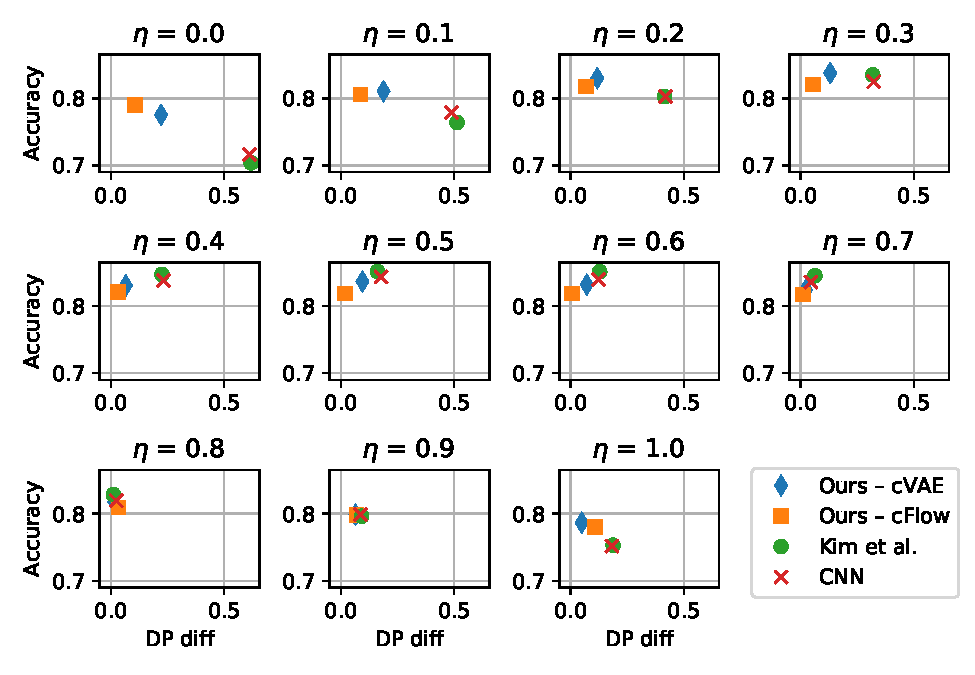
\includegraphics[width=0.85\textwidth]{paper2/Figures/nosinn_adult_multiplot_all_landscape_diff.pdf}
  \caption{
      Results for the \textsc{Adult} dataset.
      The $x$-axis corresponds to the difference in positive rates.
      An ideal result would occupy the \textsc{top-left}.
  }%
  \label{fig:big-adult-chart}
\end{figure}
\begin{figure}[htb]
    \centering
    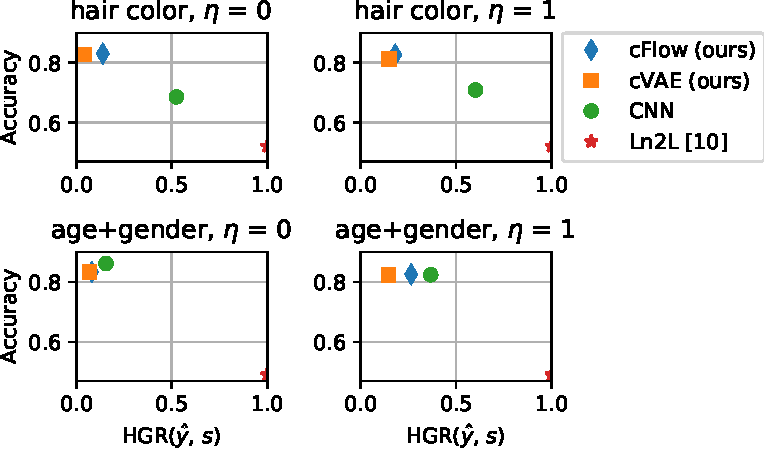
\includegraphics[width=0.7\textwidth]{paper2/Figures/celeba_multi_s.pdf}
    \caption{
        For \emph{hair colour}, $s$ takes on the values Blond, Brown and Black.
        For \emph{age+gender}, $s$ takes on the values Young/Female, Young/Male, Old/Female and Old/Male.
    }%
    \label{fig:multi-s}
\end{figure}

\paragraph{Multinomial sensitive attributes.}
In addition to binary sensitive attribute $s$,
we also investigate multinomial $s$ in the CelebA dataset.
First, we do experiments with hair colour, where $s$ has three possible values:
blond hair, brown hair and black hair.
The other experiment is with a combination of age and gender,
where $s$ has four possible values, each of which is a combination of a gender and an age:
Young/Female, Young/Male, Old/Female and Old/Male.
To evaluate the fairness for multinomial $s$, we use the Hirschfeld-Gebelein-R\'enyi Maximum Correlation Coefficient (HGR) \citep{mary2019fairness} that is defined on the domain $[0, 1]$ and gives $\text{HGR}(Y,S)=0$ iff $Y \perp S$
and 1 if there is a deterministic function to map between them.
Results can be found in figure~\ref{fig:multi-s}.\\

\begin{table}[tp]
\caption{Results on the CelebA dataset with different sizes of $z_b$.}
    \label{tab:zs-ablation}
    \centering
\begin{tabular}{l@{\extracolsep{1cm}}lrr}
\toprule
 $|z_b|$ & $|z_b|/|z|$ &  Accuracy &   DP diff \\
\midrule
          1 &             0.0082\% &  0.60 &  0.63 \\
          3 &             0.0245\% &  0.60 &  0.63 \\
          5 &             0.0410\% &  0.84 &  0.12 \\
         10 &             0.0820\% &  0.84 &  0.12 \\
         30 &             0.2442\% &  0.74 &  0.23 \\
         50 &             0.4070\% &  0.68 &  0.27 \\
\bottomrule
\end{tabular}
\end{table}
\noindent\textsc{Investigation into the size of $z_b$.}
\;\; In the cFlow model, the size of $z_b$ is an important hyperparameter which can affect the result significantly.
Here we investigate the sensitivity of the model to the choice of $z_b$ size.
Table~\ref{tab:zs-ablation} shows accuracy and fairness (as measured by \emph{DP diff}) for different sizes of $z_b$.
The results show that both too large and too small $z_b$ is detrimental.
However, they also show that the model is not overly sensitive to this parameter:
both sizes 5 and 10 achieve nearly identical results.

\begin{table}[tbp]
    \caption{
        Additional fairness metrics for the experiments on the CelebA dataset (fig.~\ref{fig:celeba-multiplot} from the main text).
        \emph{TPR diff.}\ refers to the difference in true positive rate.
        \emph{TNR diff.}\ refers to the difference in true negative rate.
        \textsc{Left:} $\eta = 0$. \textsc{Right:} $\eta=1$.
    }
    \label{tab:my_label}
    \resizebox{.49\textwidth}{!}{
    \begin{tabular}{lrrrr}
\toprule
     Method &  Accuracy &  DP diff &  TPR diff &  TNR diff \\
\midrule
      cFlow &      0.83 &     0.10 &      0.15 &      0.25 \\
       cVAE &      0.82 &     0.05 &      0.09 &      0.18 \\
        CNN &      0.61 &     0.63 &      0.70 &      0.64 \\
 Ln2L &      0.52 &     0.00 &      0.00 &      0.00 \\
\bottomrule
\end{tabular}}
\hfill
\resizebox{.49\textwidth}{!}{
\begin{tabular}{lrrrr}
\toprule
     Method &  Accuracy &  DP diff &  TPR diff &  TNR diff \\
\midrule
      cFlow &      0.82 &     0.33 &      0.28 &      0.21 \\
       cVAE &      0.81 &     0.16 &      0.10 &      0.05 \\
        CNN &      0.67 &     0.75 &      0.66 &      0.76 \\
Ln2L &      0.51 &     0.08 &      0.06 &      0.09 \\
\bottomrule
\end{tabular}}
\end{table}
\paragraph{Additional fairness metrics.}
In addition to \emph{DP diff}, we report here the result from other fairness measures.
These results are from the same setup as those reported in the main paper.
We report the difference in true positive rates (TPR) between the two groups (male and female), which corresponds to a measure of Equality of Opportunity,
and the difference in true negative rates (TNR) between the two groups.

\subsection{Optimisation Details}\label{sec:optimisation-details}
\noindent All our models were trained using the RAdam optimiser \citep{liu2019variance} with learning rates $3\times10^{-4}$ and $1\times10^{-3}$ for the encoder/discriminator pair and classifier respectively. A batch size of 128 was used for all experiments.

We now detail the optimisation settings, including the choice of adversary, specific to each dataset. Details of the cVAE and cFlow architectures can be found in table \ref{tab:vae_architectures} and table \ref{tab:inn_architectures}, respectively.

\paragraph{UCI Adult.} 
For this dataset our experiment benefited from using null-samples as inputs to the adversary of the cFlow model. Unlike for the image datasets, we found a single adversary to be sufficient. This was realised as a multi-layer perceptron (MLP) with one hidden layer, 256 units wide. The INN performs a bijection of the form $f: \mathbb{R}^n \rightarrow \mathbb{R}^n$. However, the adult dataset is composed of mostly discrete (binary/categorical) features. To achieve good performance, we found it necessary to first pre-process the inputs with a pretrained autoencoder, using its encodings as the input to the cFlow model, as well as to the adversary. The learned representations were evaluated with a logistic regression model from scikit-learn \citep{scikit-learn}, using the standard settings. All baseline models were trained for 200 epochs.
The Ln2L \citep{kim2019learning} and MLP baselines share the architecture of the cVAE's encoder, only with a classification layer affixed.

\paragraph{Coloured MNIST.}
Each level of the architecture used for the downstream classifier and na\"ive baseline alike consists of two convolutional layers, each with kernel size 3 and followed by Batch Norm \citep{ioffe2015batch} and ReLU activation. For the Ln2L baseline, we use an a setup identical to that described in \citet{kim2019learning}. Each level has twice the number of filters in its convolutional layer and half the spatial input dimensions as the last. The original input is downsampled to the point of the output being reduced to a vector, to which a fully-connected classification layer is applied.

To allow for an additional level in the INN (the downsampling operations requiring the number of spatial dimensions to be even), the data was zero-padded to a size of $32\times32$. The cVAE and cFlow models were trained for 50 and 200 epochs respectively, using $\ell_2$ reconstruction loss for the former. The downstream classifier and all baselines were trained for 40 epochs. For both of our models, an ensemble of 5 adversaries was applied to the encodings, with each member taking the form of a fully-connected ResNet, 2 blocks in depth, with SeLU activation \citep{klambauer2017self}. The adversaries were reinitialised independently with probability $0.2$ at the end of each epoch. While the adversaries could equally well take  null-samples as input, as done for the Adult dataset, doing so requires the performing of both forward and inverse passes each iteration, which, for the convolutional INNs of the depths we require for the image datasets, introduces a large computational overhead, while also showing to be the less stable of the two approaches in our preliminary experiments.

\paragraph{CelebA.} 
The downstream classifier and na\"ive baseline take the same form as described above for cMNIST, but with an additional level with 32 filters in each of its convolutions at the top of the network. For this dataset we adapt the Ln2L model by simply considering it as an augmentation the na\"ive baseline's objective function, with the entropy loss applied to the output of the final convolutional layer. These models were again trained for 40 epochs, which we found to be sufficient for convergence for the tasks in question. The cVAE and cFlow models were respectively trained for 100 epochs and 30 epochs, using $\ell_1$ reconstruction loss for the former. Compared with cMNIST, the size of the adversarial ensemble was increased to 10, the reinitialisation probability to 0.33, but no changes were made to the architectures of its members.

\paragraph{The Pitfalls of Adversarial Training.}
Adversarial learning has become one of the go-to methods for enforcing invariance in fair representation learning \citep{ganin2016domain} with MMD \citep{louizos2016variational} and HSIC \citep{QuaShaTho19}, being popular non-parametric alternatives.
\citet{ganin2016domain} proposed adversarial learning for domain adaptation problems, with \citet{edwards2016censoring} soon after making this and learning a representation promoting demographic parity.
The adversarial approach carries the benefits of being both efficient and scalable to multi-class categorical variables, which many sensitive attributes are in practice, whereas the non-parametric methods only permit pair-wise comparison.

However, when realised as a neural network, the adversary is both sensitive to the values of the inputs as well as their ordering (though exchangeable architectures, such as \citet{zaheer2017deep} do exist, but which sacrifice expressiveness).
Thus, it can happen that the representation learner optimises for the surrogate objective of eluding the adversary rather than the real objective of expelling $s$-related information.
Moreover, the non-stationarity of the dynamics can lead to cyclic-equilibria, irrespective of the capacity of the adversary.

When working with a partitioned latent space, this behaviour can be averted by instead encouraging $z_b$ to be predictive of $s$, acting as a kind of information ``sink``, as in \citet{JacSmeOya18}.
However, this does not have the guarantee of making $z_u$ invariant to $s$ - there are often many indicators for $s$, not all of which are needed to predict the label perfectly.
Training the network to convergence before taking each gradient step with the representation learner is one way one to attempt to tame the unstable minimax dynamics \citep{feng2019learning}.
However, this does not prevent the emergence of the aforementioned cyclicity.

We try to mitigate the aforementioned degeneracies by maintaining a diverse set of adversaries, as has shown to be effective for GAN training \citep{durugkar2016generative}, and by decorrelating the individual trajectories by intermittently re-initialising them with some small probability following each iteration.

\paragraph{Tuning the Partition Sizes.}
There are several ways of ensuring that the size of $z_b$ is sufficient to capture all s dependencies, but minimal enough that information unrelated to s is maximally preserved
We adopt the straightforward search strategy of, starting from some initial guess, calibrating the value according to accuracy attained by a classifier trained to predict $s$ from $z_b$ on a held-out subset of the representative set, which is measured whenever the adversarial loss plateaus. If the accuracy is above chance level then that suggests the size of the $z_b$ partition, $|z_b|$, needs to be increased to accommodate more information about $s$. If the accuracy is found to be at chance level then are two possibilities: 1) $|z_b|$ is already optimal; 2) $|z_b|$ is large enough that it fully contains both information $s$ as well as that of a portion of $y$. If the former is true, then perturbations around the current value allow us to confirm this; if the latter is true then decreasing the value was indeed the correct decision.

\subsection{Synthesising Coloured MNIST}\label{sec:color-details}
\noindent We use a colourised version of MNIST as a controlled setting investigate learning from biased data in the image domain. In the biased training set, each digit is assigned a unique mean RGB value parameterising the multivariate Gaussian from which its colour is drawn. These values were chosen to be maximally dispersed across the 8-bit colour spectrum and are listed in table \ref{tab:cmnist_rgb_values}. By adjusting the standard deviation, $\sigma$, of the Gaussians, we adjust the degree of bias in the dataset. When $\sigma=0$, there is a perfect and noiseless correspondence between colour and digit class which a classifier can exploit. The classifier can favour the learning of the low-level spurious feature over those higher level features constituent of the digit's class. As the standard deviation increases, the sampled RGB values are permitted to drift further from the mean, leading to overlap between the samples of the colour distributions and reducing their reliability as indicators of the digit class. In the test and representative sets alike, however, the colour of each sample is sampled from one of the 10 distributions randomly, such that colour can no longer be leveraged as a shortcut to predicting the digit's class.

\subsection{Stabilising the Coupling layers}\label{sec:those-darn-coupling-layers}
\noindent Heuristically, we found that  applying an additional nonlinear function to the scale coefficient of the form
\begin{align}
  s = \sigma (f(u)) + 0.5
  \label{eq:heuristic-1}
\end{align}
greatly improved the stability of the affine coupling layers. Here, $\sigma$ is the logistic function, which we shift to be centred on 1 so that zero-initialising $f$ results in the coupling layers initially performing an identity-mapping.

\begin{table}[tp]
\caption{Mean RGB values (in practice normalised to $[0, 1]$) parameterising the Multivariate Gaussian distributions from which each digit's colour is sampled in the biased (training) dataset. In the representative and test sets,  the colour of each digit is sampled from one of the specified Gaussian distributions at random.}
\label{tab:cmnist_rgb_values}
\centering
\begin{tabular}{l@{\extracolsep{1cm}}lll}
\toprule
Digit & Colour Name & Mean RGB      \\ \midrule
0     & Cyan        & (0, 255, 255) \\
1     & Blue        & (0, 0, 255)   \\
2     & Magenta     & (255, 0, 255) \\
3     & Green       & (0, 128, 0)   \\
4     & Lime        & (0, 255, 0)   \\
5     & Maroon      & (128, 0, 0)   \\
6     & Navy        & (0, 0, 128)   \\
7     & Purple      & (128, 0, 128) \\
8     & Red         & (255, 0, 0)   \\
9     & Yellow      & (255, 255, 0) \\ \bottomrule
\end{tabular}
\end{table}

\subsection{Qualitative Results for CelebA}\label{sec:qual-results-celeba}
\noindent Learning a representation alongside its inverse mapping, be it approximate or exact, enables us to probe the behaviour of the model that produced it,
and any biases it may have implicitly captured due to entanglement between the sensitive attribute and other attributes present in the data.
We highlight a few examples of such biases manifesting in the cFlow model's CelebA null-samples in fig.~\ref{fig:celeba_cflow_suppmat}. In these cases, makeup and hair style have been inadvertently modified during the null-sampling due to the tight correlation between these two attributes and the sensitive attribute, gender, to which we had aimed to make our representations invariant. Additionally, in all highlighted images, the skin tone has changed: from male to gender-neutral, the skin becomes lighter and from female to gender-neutral, the skin becomes darker; in the change from male to gender-neutral, glasses are also often removed.
As the model cannot know that the label is meant to only refer to gender, and not to these other (correlated) attributes,
the links cannot be disentangled by the model.
However, the advantage of our method is that we can at least identify such biases due to the interpretability that comes with the representations being in the data domain.

% \newpage
\begin{figure*}[tb]
  \centering
  \subfloat[Original images.]{%
      \scalebox{0.3}{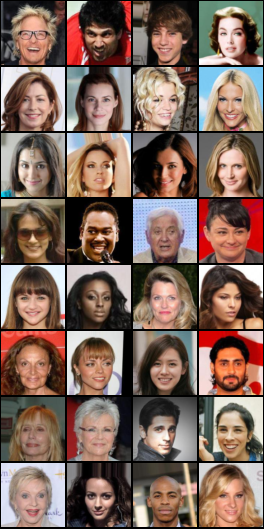
\includegraphics[width=\textwidth]{paper2/Images/celeba/vae_x_original.png}}%
      \label{fig:cvae_celeba_original_x}
  }
  \hfill
  \subfloat[$\bm{x}_u$ null-samples generated by the cVAE model.]{%
      \scalebox{0.3}{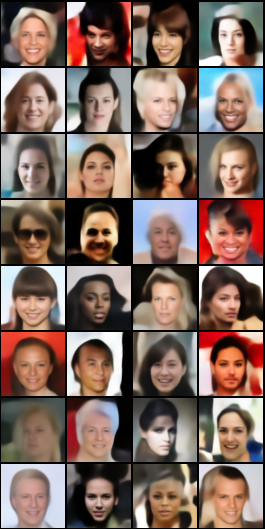
\includegraphics[width=\textwidth]{paper2/Images/celeba/vae_recon_y.png}}%
      \label{fig:cvae_celeba_recon_y}
  }
  \hfill
  \subfloat[$\bm{x}_b$ null-samples generated by the cVAE model.]{%
      \scalebox{0.3}{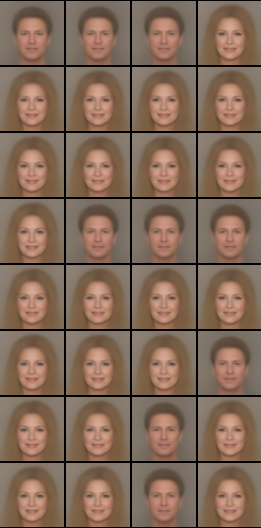
\includegraphics[width=\textwidth]{paper2/Images/celeba/vae_recon_s.png}}%
      \label{fig:cvae_celeba_recon_s}
  }
  \caption{
    CelebA null-samples learned by our cVAE model, with gender as the sensitive attribute.
    (a) The original, untransformed samples from the CelebA dataset
    (b) Reconstructions using only information unrelated to $s$.
    (c) Reconstruction using only information related to $\neg s$.
    The model learns to disentangle gender from the non-gender related information. Compared with the cFlow model, there is a severe degradation in reconstruction quality due to the model trying to simultaneously satisfy conflicting objectives.
    % Attributes such as \emph{makeup} and \emph{hair length} are also often modified in the process due to inherent correlations between them and the sensitive attribute, which the intepretability of our representations allows us to easily identify.
  }\label{fig:celeba_vae}
\end{figure*}

\begin{figure*}[tb]
  \centering
  \subfloat[Original images.]{%
      \scalebox{0.3}{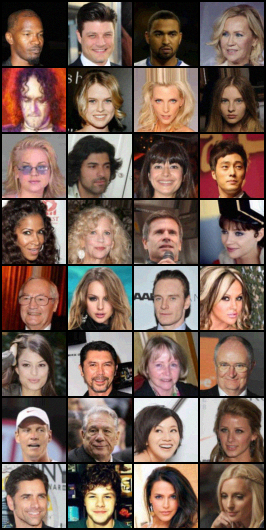
\includegraphics[width=\textwidth]{paper2/Images/celeba/cflow_original_x_suppmat.png}}%
      \label{fig:cflow_celeba_original_x_suppmat}
  }
  \hfill
  \subfloat[$\bm{x}_u$ null-samples generated by the cFlow model.]{%
      \scalebox{0.3}{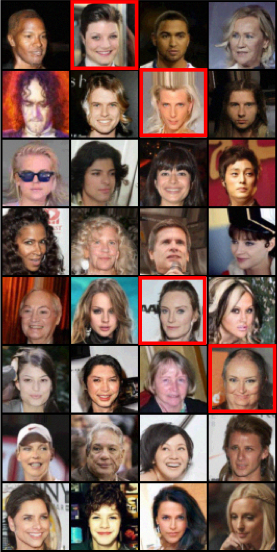
\includegraphics[width=\textwidth]{paper2/Images/celeba/cflow_xd_suppmat.png}}%
      \label{fig:cflow_celeba_recon_y_suppmt}
  }
  \hfill
  \subfloat[$\mathbf{x}_b$ null-samples generated by the cFlow model.]{%
      \scalebox{0.3}{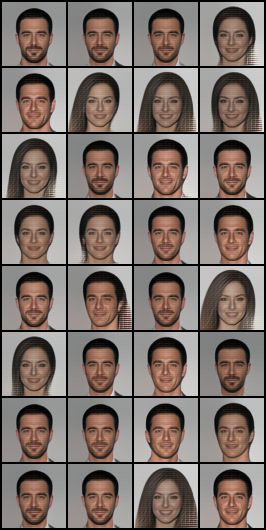
\includegraphics[width=\textwidth]{paper2/Images/celeba/cflow_xb_suppmat.png}}%
      \label{fig:cflow_celeba_recon_s_suppmat}
  }
  \caption{
    CelebA null-samples learned by our cFlow model, with gender as the sensitive attribute.
    (a) The original, untransformed samples from the CelebA dataset
    (b) Reconstructions using only information unrelated to $s$.
    (c) Reconstruction using only information related to $\neg s$.
    The model learns to disentangle gender from the non-gender related information.
    Attributes such as \emph{makeup} and \emph{hair length} are also often modified in the process (prime examples framed with red) due to inherent correlations between them and the sensitive attribute, which the interpretability of our representations allows us to easily identify.
  }\label{fig:celeba_cflow_suppmat}
\end{figure*}



\subsection{Transfer Learning}\label{sec:transfer-learning}
For our method, we require a representative set which follows the same distribution as that observed during deployment.
Such a representative set might not always be available.
In such a scenario, we can resort to using a set that is merely \emph{similar} to that in the deployment setting and leverage transfer learning.

%We argue that the inherent properties of INNs make them especially suitable for transfer learning.
One of the advantages of using an invertible architecture over conventional, \emph{surjective} ones that we stressed in the main text is its \emph{losslessness}. Since the transformations are necessarily bijective, the information contained in the input can never be destroyed, only redistributed. This makes such models particularly well-suited, in our minds, for transferring learned invariances:
even if the input is unfamiliar, no information should be lost when trying to transform it.
This works as long as only the information about $s$ ends up in the $z_b$ partition.
If $s$ takes a form similar to that which we pre-trained on, and can thus be correctly partitioned in the latent space, by complement we have the information about $\neg s$ stored in the $z_u$ partition, without presupposing similarity to the $\neg s$ observed during pre-training.

\paragraph{Transferring from mixed-NIST to MNIST.}
We test our hypothesis by comparing the performance of the cFlow and cVAE models pre-trained on a mixture of datasets belonging to the NIST family, colourised in the same way as cMNIST, while the downstream train and test sets remain the same as in the original cMNIST experiments. Specifically, we create this representative set by sampling 24,000 images (to match the cardinality of the original representative set) from EMNIST (letters only)~\citep{cohen2017emnist}, Fashion\-MNIST~\citep{xiao2017fashion} and KMNIST~\citep{clanuwat2018deep}, in equal proportion. We use the same architectures for the cVAE and cFlow models as we did in the non-transfer learning setting. In terms of hyperparameters, the only change made was to the KL-divergence's pre-factor, finding it necessary to increase it to $1$ to guarantee stability.

The results for the range of $\sigma$ values are shown in fig.~\ref{fig:cmnist-transfer}. Unsurprisingly, the performance of both models suffers when the representative and test sets do not completely correspond. However, the cFlow model consistently outperforms the cVAE model, with the gap increasing as the bias decreases.
Although some colour information is retained in the cFlow null-samples, symptomatic of an imperfect transfer, semantic information is almost entirely retained as well.
Conversely, the cVAE is very much flawed in this respect; as can be seen in the bottom row of fig.~\ref{fig:cmnist-transfer}, for some samples, semantic information is degraded to the point of the digit's identity being altered. As a result of this semantic degradation, the performance of the downstream classifier is curtailed by the noisiness of the digit's identity and is relatively unchanging across $\sigma$-values, in contrast to the monotonic improvement of that achieved on the cFlow null-samples.
% \begin{figure}
%   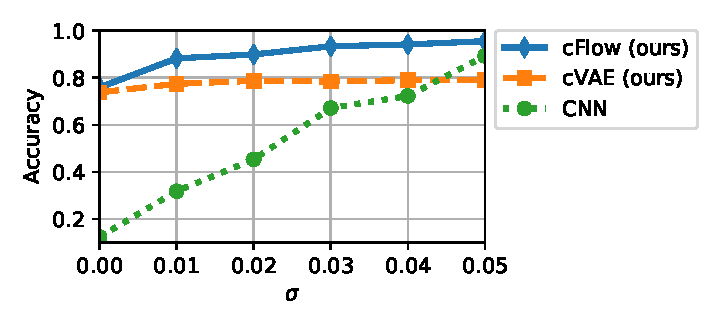
\includegraphics[width=0.6\textwidth]{paper2/Figures/nosinn_cmnist_transfer.pdf}
%   \caption{
%      Results for transfer learning experiments on cMNIST.
%   }%
%   \label{fig:cmnist-transfer}
% \end{figure}

\begin{figure*}[htb]
  \centering
  \subfloat[Performance on cMNIST test data after pre-training on the mixed NIST dataset.]{
      \scalebox{0.6}{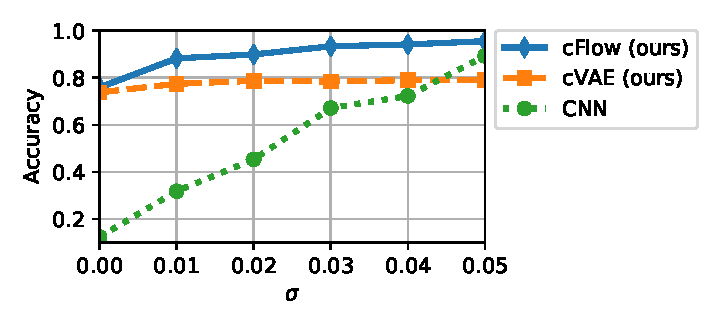
\includegraphics[width=\textwidth]{paper2/Figures/nosinn_cmnist_transfer.pdf}} \label{fig:cmnist-transfer}
  }
  %---
  \vspace{10pt}
 
  \subfloat[Test data input to the cFlow model.]{%
      \scalebox{0.3}{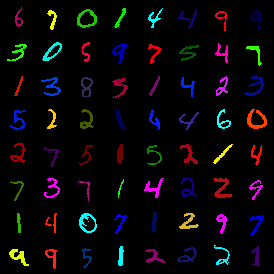
\includegraphics[width=\textwidth]{paper2/Images/cmnist/cflow_tl_original.png}}%
      \label{fig:cflow_tl_original}
  }
  ~~~
%   \hfill
  \subfloat[$\bm{x}_u$ null-samples generated by the cFlow model.]{%
      \scalebox{0.3}{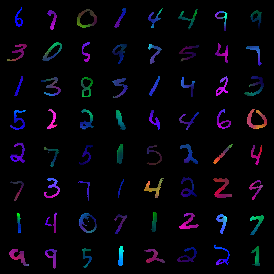
\includegraphics[width=\textwidth]{paper2/Images/cmnist/cflow_tl_xd.png}}%
      \label{fig:cflow_tl_xd}
  }
  
    \subfloat[Test data input to the cVAE model.]{%
      \scalebox{0.3}{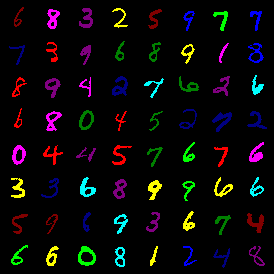
\includegraphics[width=\textwidth]{paper2/Images/cmnist/cvae_tl_original.png}}%
      \label{fig:cvae_tl_original}
  }
  ~~~
%   \hfill
  \subfloat[$\bm{x}_u$ null-samples generated by the cVAE model.]{%
      \scalebox{0.3}{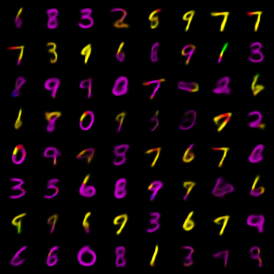
\includegraphics[width=\textwidth]{paper2/Images/cmnist/cvae_tl_xd.png}}%
      \label{fig:cvae_tl_xd}
  }
  \caption{
    Results for the transfer learning experiments in which the representative set consists of colourised samples from EMNIST, KMNIST, and FashionMNIST, while the downstream dataset remains as cMNIST. (a) Quantitative results for different $\sigma$-values. (b-c) Qualitative results for the cFlow model.
    (d-e) Qualitative results for the cVAE model. The qualitative results provide comparisons of the images before (left) and after (right) null-sampling. Note that for some of the cVAE samples, the clarity of the digits has clearly changed due to null-sampling, serving as an explanation for the non-increasing downstream performance.
  }%
  \label{fig:cmnist-transfer-all}
  
\end{figure*}

% \clearpage

% \bibliographystyle{splncs04}
% \bibliography{references.bib}

% \end{appendix}

% \end{document}

% \FloatBarrier%
% \clearpage

% \printbibliography%
% \end{refsection}

% \end{document}
